\documentclass[13pt]{extarticle}

\usepackage[a4paper, margin=2cm]{geometry}
\usepackage{graphicx}
\usepackage{enumitem}
\usepackage{caption, subcaption}
\usepackage{array}
\usepackage{tikz}
\usetikzlibrary{automata, arrows.meta, positioning}
\usepackage{titlesec}
\titleformat*{\subsubsection}{\large\bfseries}
\newcolumntype{P}[1]{>{\centering\arraybackslash}p{#1}}
\usepackage{float}

% ---------- Language + Unicode ----------
\usepackage{polyglossia}
\setmainlanguage{greek}
\setotherlanguage{english}
\usepackage{fontspec}
\newfontfamily\greekfonttt{FreeMono}
\setmainfont{Linux Libertine O}

% ---------- Start document ----------
\begin{document}

% ─────────────── Τίτλος Εργασίας ───────────────
\begin{titlepage}
    \centering

    {\huge \textbf{Εθνικό Μετσόβιο Πολυτεχνείο}}\\[0.3cm]
    {\Large Σχολή Ηλεκτρολόγων Μηχανικών και Μηχανικών Υπολογιστών}\\[2.8cm]

    % Λογότυπο κάτω από το όνομα του ΕΜΠ
    \includegraphics[width=0.4\textwidth]{emp_logo.png} \\[2.8cm]

    {\huge \textbf{Βάσεις Δεδομένων (2024–2025)}}\\[0.3cm]
    {\LARGE Pulse University Database}\\[0.8cm]
    {\Large https://github.com/ntua-el21026/DB25\_137.git}\\[2.8cm]

    % Δίστηλη διάταξη: Ομάδα αριστερά, Μάθημα δεξιά
    \noindent
    \begin{minipage}[t]{0.48\textwidth}
        \raggedright
        {\large \underline{\textbf{Στοιχεία Ομάδας - DB137}}}\\[0.4cm]
        \begin{itemize}[left=0pt,label=--]
            \item \textbf{Πέππας Μιχαήλ-Αθανάσιος}, 03121026
            \item \textbf{Τσουβαλάς Ανδρέας}, 03121022
            \item \textbf{Μάντζαρης Κωνσταντίνος}, 03122406
        \end{itemize}
    \end{minipage}
    \hfill
    \begin{minipage}[t]{0.48\textwidth}
        \raggedright
        {\large \underline{\textbf{Στοιχεία Μαθήματος}}}\\[0.4cm]
        \begin{itemize}[left=0pt,label=--]
            \item \textbf{Διδάσκοντες:} Δ. Τσουμάκος, Μ. Κόνιαρης
            \item \textbf{Εργαστήριο:} Συστημάτων Βάσεων Γνώσεων και Δεδομένων
            \item \textbf{Εξάμηνο:} Εαρινό 2025
        \end{itemize}
    \end{minipage}\\[2.5cm]

    {\large Αθήνα, Μάιος 2025}
\end{titlepage}

% ─────────────── Περιεχόμενα ───────────────
\clearpage
\tableofcontents
\clearpage
\setcounter{page}{2}

% ─────────────── 1. Εισαγωγή ───────────────
\clearpage
\section{Εισαγωγή}

Το έγγραφο αυτό περιγράφει τον σχεδιασμό, την υλοποίηση και τις λειτουργίες της βάσης δεδομένων και του συστήματος \textbf{Pulse University}, το οποίο αναπτύχθηκε στο πλαίσιο της εξαμηνιαίας εργασίας για το μάθημα \textit{Βάσεις Δεδομένων}, κατά το ακαδημαϊκό έτος 2024–2025.

Στόχος του έργου είναι η δημιουργία μιας πλήρους και ρεαλιστικής πληροφοριακής υποδομής για τη διαχείριση μουσικών φεστιβάλ, καλλιτεχνών, διοργανώσεων, επισκεπτών και στατιστικών αξιολογήσεων. Το σύστημα υποστηρίζει πολλαπλά φεστιβάλ ανά έτος και ήπειρο, διαχείριση χωρητικότητας, προγραμματισμό εμφανίσεων και δυναμικό μηχανισμό εισιτηρίων με αγοραπωλησίες, ουρές, και αξιολογήσεις.\\

Η ανάπτυξη καλύπτει:
\begin{itemize}
  \item Τον σχεδιασμό και την υλοποίηση ενός σχεσιακού σχήματος σε MySQL, με αυστηρούς περιορισμούς ακεραιότητας και triggers για την επιβολή επιχειρησιακών κανόνων.
  \item Την ανάπτυξη εφαρμογής γραμμής εντολών (\texttt{CLI}) για την πλήρη διαχείριση του σχήματος, των χρηστών, και των ερωτημάτων.
  \item Την κατασκευή μιας σύγχρονης frontend SPA εφαρμογής (React + Tailwind), που επιτρέπει τη διεπαφή με τη βάση μέσω γραφικών καρτελών, επεξεργαστή SQL, και εργαλείων CLI.
  \item Την αυτοματοποιημένη παραγωγή συνθετικών δεδομένων μέσω Python scripts που σέβονται όλα τα triggers και τους περιορισμούς της βάσης.
  \item Την αξιολόγηση της απόδοσης και της κάλυψης ερωτημάτων μέσω indexing, views, και σχετικών metrics.
\end{itemize}

Η προσέγγιση που ακολουθήθηκε βασίζεται στην επεκτασιμότητα, την αναπαραγωγιμότητα και την αυστηρή διασφάλιση ακεραιότητας δεδομένων, με στόχο τη δημιουργία ενός συστήματος που μπορεί να δοκιμαστεί, να επεκταθεί και να χρησιμοποιηθεί παραγωγικά σε οποιδήποτε περιβάλλον.

\subsection{Δομή του Project}

Η δομή του project ακολουθεί μία καθαρή και κατανοητή οργάνωση, βασισμένη στη διάκριση λειτουργικών ενοτήτων του συστήματος. Κάθε φάκελος εξυπηρετεί συγκεκριμένο σκοπό, ενώ διατηρείται συνοχή μεταξύ τεκμηρίωσης, υλοποίησης και δοκιμών.

\noindent\textbf{Ριζική Δομή Φακέλων:}
\begin{verbatim}
.
├── cli/               # Διεπαφή γραμμής εντολών (CLI) - διαχείριση DB και χρηστών
│   ├── db137.py       # Κύριο CLI script με τις εντολές
│   └── users/         # Υποσύστημα διαχείρισης χρηστών/endpoint
├── code/              # Βοηθητικά scripts για παραγωγή δεδομένων, οργάνωση, και εργαλεία κώδικα
│   ├── data_generation/   # Συνθετικά δεδομένα (faker.py, faker_sql.py)
│   ├── code_utils/        # Εργαλεία για queries και consistency checks (qgen.py κ.ά.)
│   └── organization/      # Ανάλυση/δομή αρχείων έργου (struct.py)
├── diagrams/          # ER και relational διαγράμματα (PDF)
├── docs/              # Αναφορά, εκφώνηση και εσωτερική τεκμηρίωση
├── frontend/          # Περιβάλλον web (React/Vite) με tabs: Schema, Browse, Query, CLI
│   ├── public/            # Δημόσια assets (π.χ. logo)
│   ├── src/
│   │   ├── api/           # Διαχείριση επικοινωνίας με Flask backend
│   │   ├── auth/          # Ενότητες authentication (login, session storage)
│   │   ├── components/    # Επαναχρησιμοποιήσιμα στοιχεία UI (π.χ. session timer)
│   │   ├── hooks/         # Custom React hooks (π.χ. useSchema)
│   │   ├── pages/         # Δομή σελίδων (π.χ. LoginPage, MainPage)
│   │   ├── tabs/          # Περιεχόμενο των καρτελών του UI (Schema, CLI, Query, Browse)
│   │   ├── App.jsx        # Root component
│   │   ├── main.jsx       # Entry point εφαρμογής
│   │   └── index.css      # Tailwind styling
│   ├── index.html         # HTML πρότυπο της εφαρμογής
│   ├── tailwind.config.js # Ρυθμίσεις Tailwind
│   └── vite.config.js     # Ρυθμίσεις Vite
├── sql/               # SQL scripts (install, triggers, indexes, views, procedures)
│   └── queries/       # Υλοποιήσεις Q01–Q15 και αποτελέσματα (QXX_out.txt, plans)
├── test/              # Scripts αυτόματων δοκιμών CLI (test_cli.sh)
└── .envrc             # Περιβάλλον χρήστη (DB credentials, path setup)
\end{verbatim}

\noindent\textbf{Επεξήγηση βασικών φακέλων:}
\begin{itemize}
  \item \texttt{cli/}: Περιέχει το βασικό εργαλείο γραμμής εντολών \texttt{db137.py}, το οποίο υλοποιεί όλες τις λειτουργίες διαχείρισης της βάσης: δημιουργία/διαγραφή/φόρτωση, reset, εκτέλεση ερωτημάτων, καθώς και εντολές για χρήστες. Το υποσύστημα \texttt{users/manager.py} είναι υπεύθυνο για τη σύνδεση με τη MySQL και τον χειρισμό χρηστών και δικαιωμάτων.

  \item \texttt{code/}: Περιέχει scripts που υποστηρίζουν την παραγωγή, τον έλεγχο και την ανάλυση δεδομένων:
  \begin{itemize}
    \item \texttt{data\_generation/}: Περιλαμβάνει τους δύο τρόπους παραγωγής δεδομένων:
    \begin{itemize}
      \item \texttt{faker.py}: Εκτελεί εισαγωγή δεδομένων απευθείας στη βάση, σε συμμόρφωση με triggers και constraints.
      \item \texttt{faker\_sql.py}: Δημιουργεί trigger-safe SQL dump για φόρτωση offline μέσω \texttt{load.sql}.
    \end{itemize}
    \item \texttt{code\_utils/}: Scripts για αυτόματη δημιουργία ερωτημάτων και ελέγχους αρχείων, όπως:
    \begin{itemize}
      \item \texttt{qgen.py}: Δημιουργία queries και αποτελεσμάτων.
      \item \texttt{fixeof.py}, \texttt{dropgen.py}: Επεξεργασία και διόρθωση τερματισμού αρχείων ή constraints.
    \end{itemize}
    \item \texttt{organization/}: Περιλαμβάνει το \texttt{struct.py}, που αναλύει και ελέγχει τη συνοχή της δομής του έργου.
  \end{itemize}

  \item \texttt{sql/}: Κεντρικός φάκελος με όλο το SQL schema και τα graded ερωτήματα:
  \begin{itemize}
    \item \texttt{install.sql}: Ορίζει όλες τις οντότητες και τους περιορισμούς.
    \item \texttt{indexing.sql}, \texttt{triggers.sql}, \texttt{procedures.sql}, \texttt{views.sql}: Εξειδικευμένα αρχεία με indexes, triggers (33), stored procedures (7) και views.
    \item \texttt{queries/}: Αρχεία \texttt{Q01.sql} έως \texttt{Q15.sql} και τα αντίστοιχα outputs, με επιπλέον εκδοχές για trace (π.χ. \texttt{Q04\_plan1\_out.txt}).
  \end{itemize}

  \item \texttt{frontend/}: SPA εφαρμογή σε React 18 + Vite, με Tailwind CSS και shadcn/ui για μοντέρνο UI. Περιλαμβάνει:
  \begin{itemize}
    \item \texttt{src/pages/}, \texttt{src/tabs/}: Καρτέλες του UI για Schema Overview, Browse Schema, Run Query και Run CLI.
    \item \texttt{src/api/}: API client για επικοινωνία με Flask backend.
    \item \texttt{src/auth/}, \texttt{src/hooks/}: Authentication flow και custom hooks.
    \item \texttt{index.html}, \texttt{main.jsx}, \texttt{App.jsx}: Root αρχεία της εφαρμογής.
  \end{itemize}

  \item \texttt{docs/}: Φάκελος τεκμηρίωσης, με:
  \begin{itemize}
    \item \texttt{assignment.pdf}: Επίσημη εκφώνηση.
    \item \texttt{ddl.pdf}: Περιγραφή των SQL αρχείων.
    \item \texttt{report.pdf}: Η παρούσα αναφορά της εργασίας μας.
    \item \texttt{organization/}: Αναφορές σε συμμετοχές, δομή, δεδομένα (\texttt{project\_structure.txt}, \texttt{db\_data.txt}).
  \end{itemize}

  \item \texttt{diagrams/}: ER και σχεσιακά διαγράμματα της βάσης, σε μορφή PDF για εύκολη επισκόπηση.

  \item \texttt{test/}: Περιλαμβάνει το \texttt{test\_cli.sh}, ένα script που ελέγχει όλες τις CLI λειτουργίες και εξάγει συγκεντρωτικά αποτελέσματα (\texttt{test\_cli\_results.txt}).

  \item \texttt{.envrc}: Ορισμός περιβαλλοντικών μεταβλητών (π.χ. DB credentials, Python path).
\end{itemize}

\vspace{1em}
\noindent\textbf{Στόχοι σχεδιασμού:}
\begin{itemize}
  \item Ο πλήρης λειτουργικός διαχωρισμός μεταξύ backend (SQL schema, CLI logic) και frontend (SPA user interface).
  \item Η ακεραιότητα των δεδομένων, με πολυάριθμα triggers και χρήση constraints, ώστε κάθε εισαγωγή και αλλαγή να συμμορφώνεται πλήρως με το schema.
  \item Η δυνατότητα εύκολης επέκτασης και debugging μέσω εργαλείων δομής και εργαλείων κώδικα (π.χ. \texttt{struct.py}, \texttt{dropgen.py}).
  \item Η δυνατότητα εύκολης αξιολόγησης queries και ελέγχου αποτελεσμάτων για benchmarking (με χρήση \texttt{\_out.txt}, indexing.sql και views).
\end{itemize}


% ─────────────── 2. Σχεδιασμός Βάσης Δεδομένων ───────────────
\clearpage
\section{Σχεδιασμός Βάσης Δεδομένων - ER \& Relational}
\subsection{Διάγραμμα Οντοτήτων και Συσχετίσεων - ER}
\begin{center}
    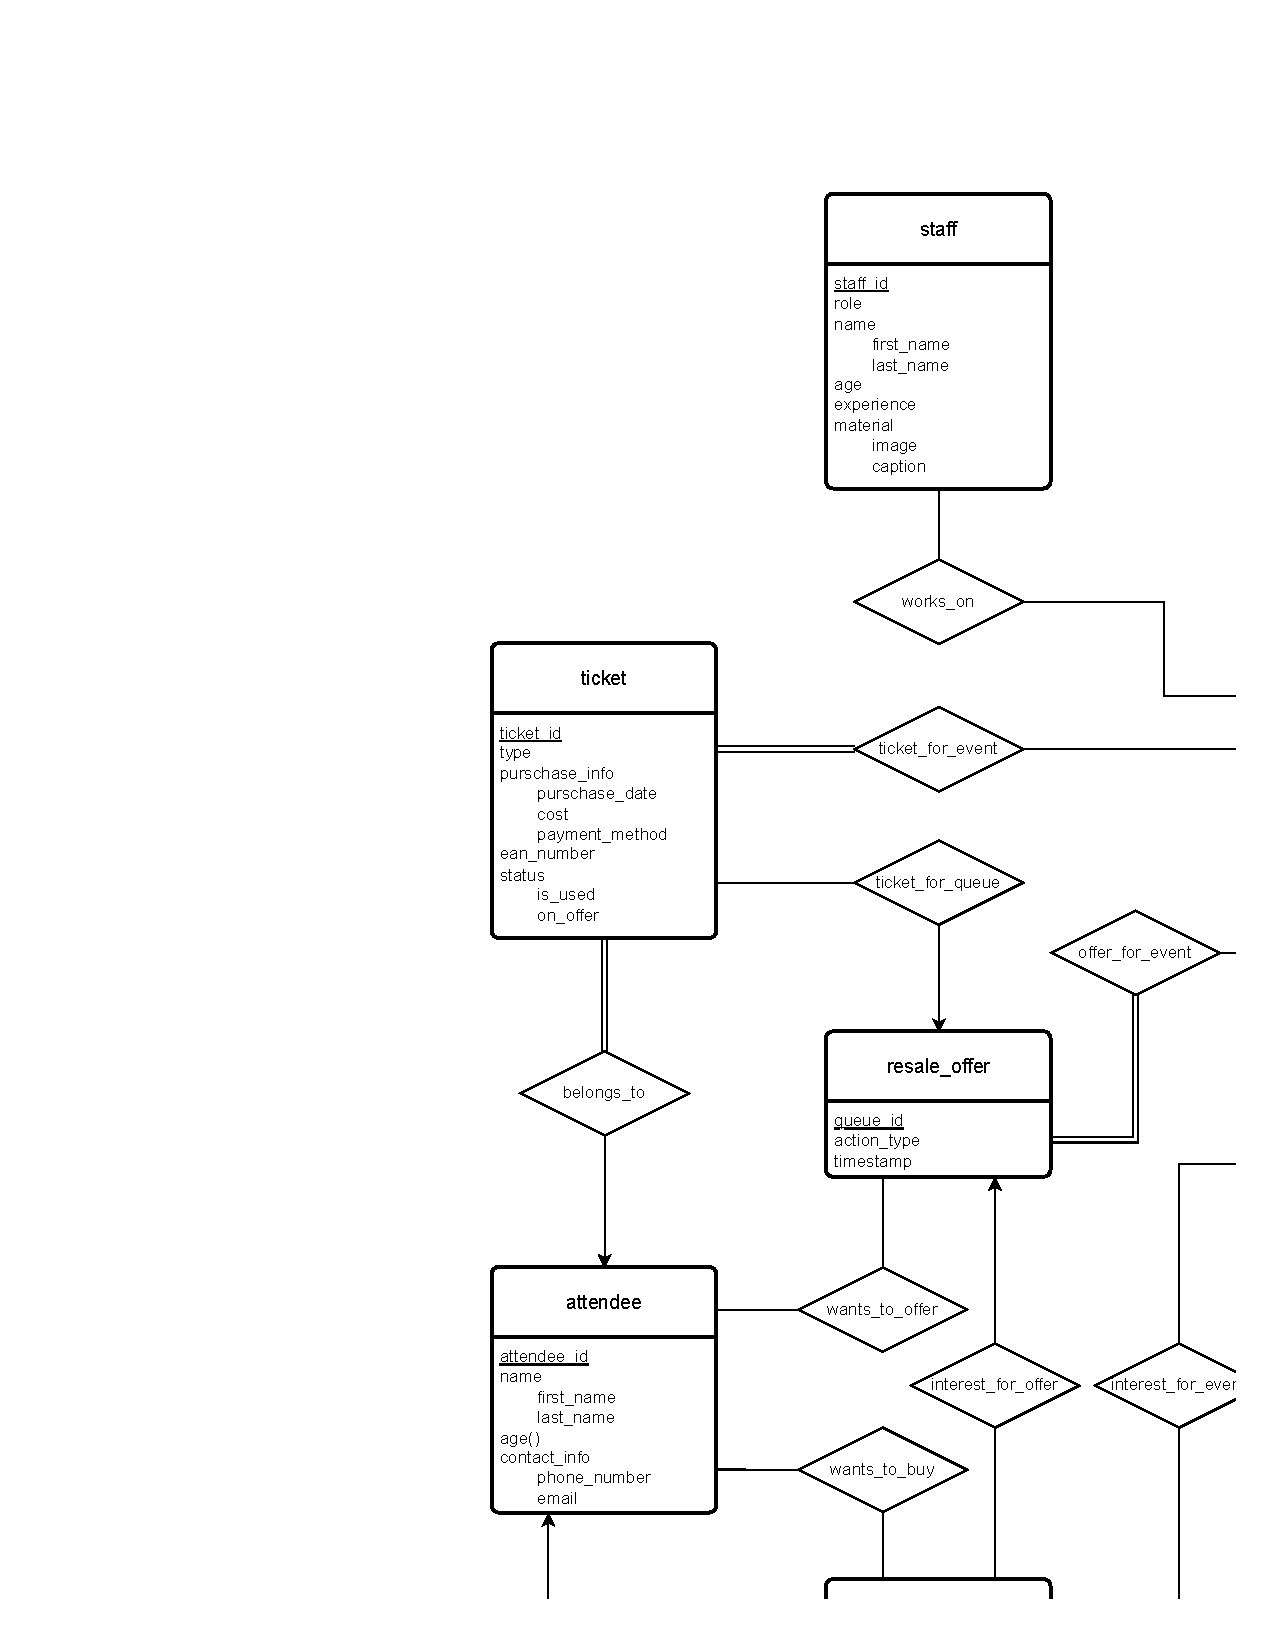
\includegraphics[width=\textwidth]{er.pdf}
\end{center}
\vspace{5cm}

\subsection{Σχεσιακό Μοντέλο - Relational}
\begin{center}
    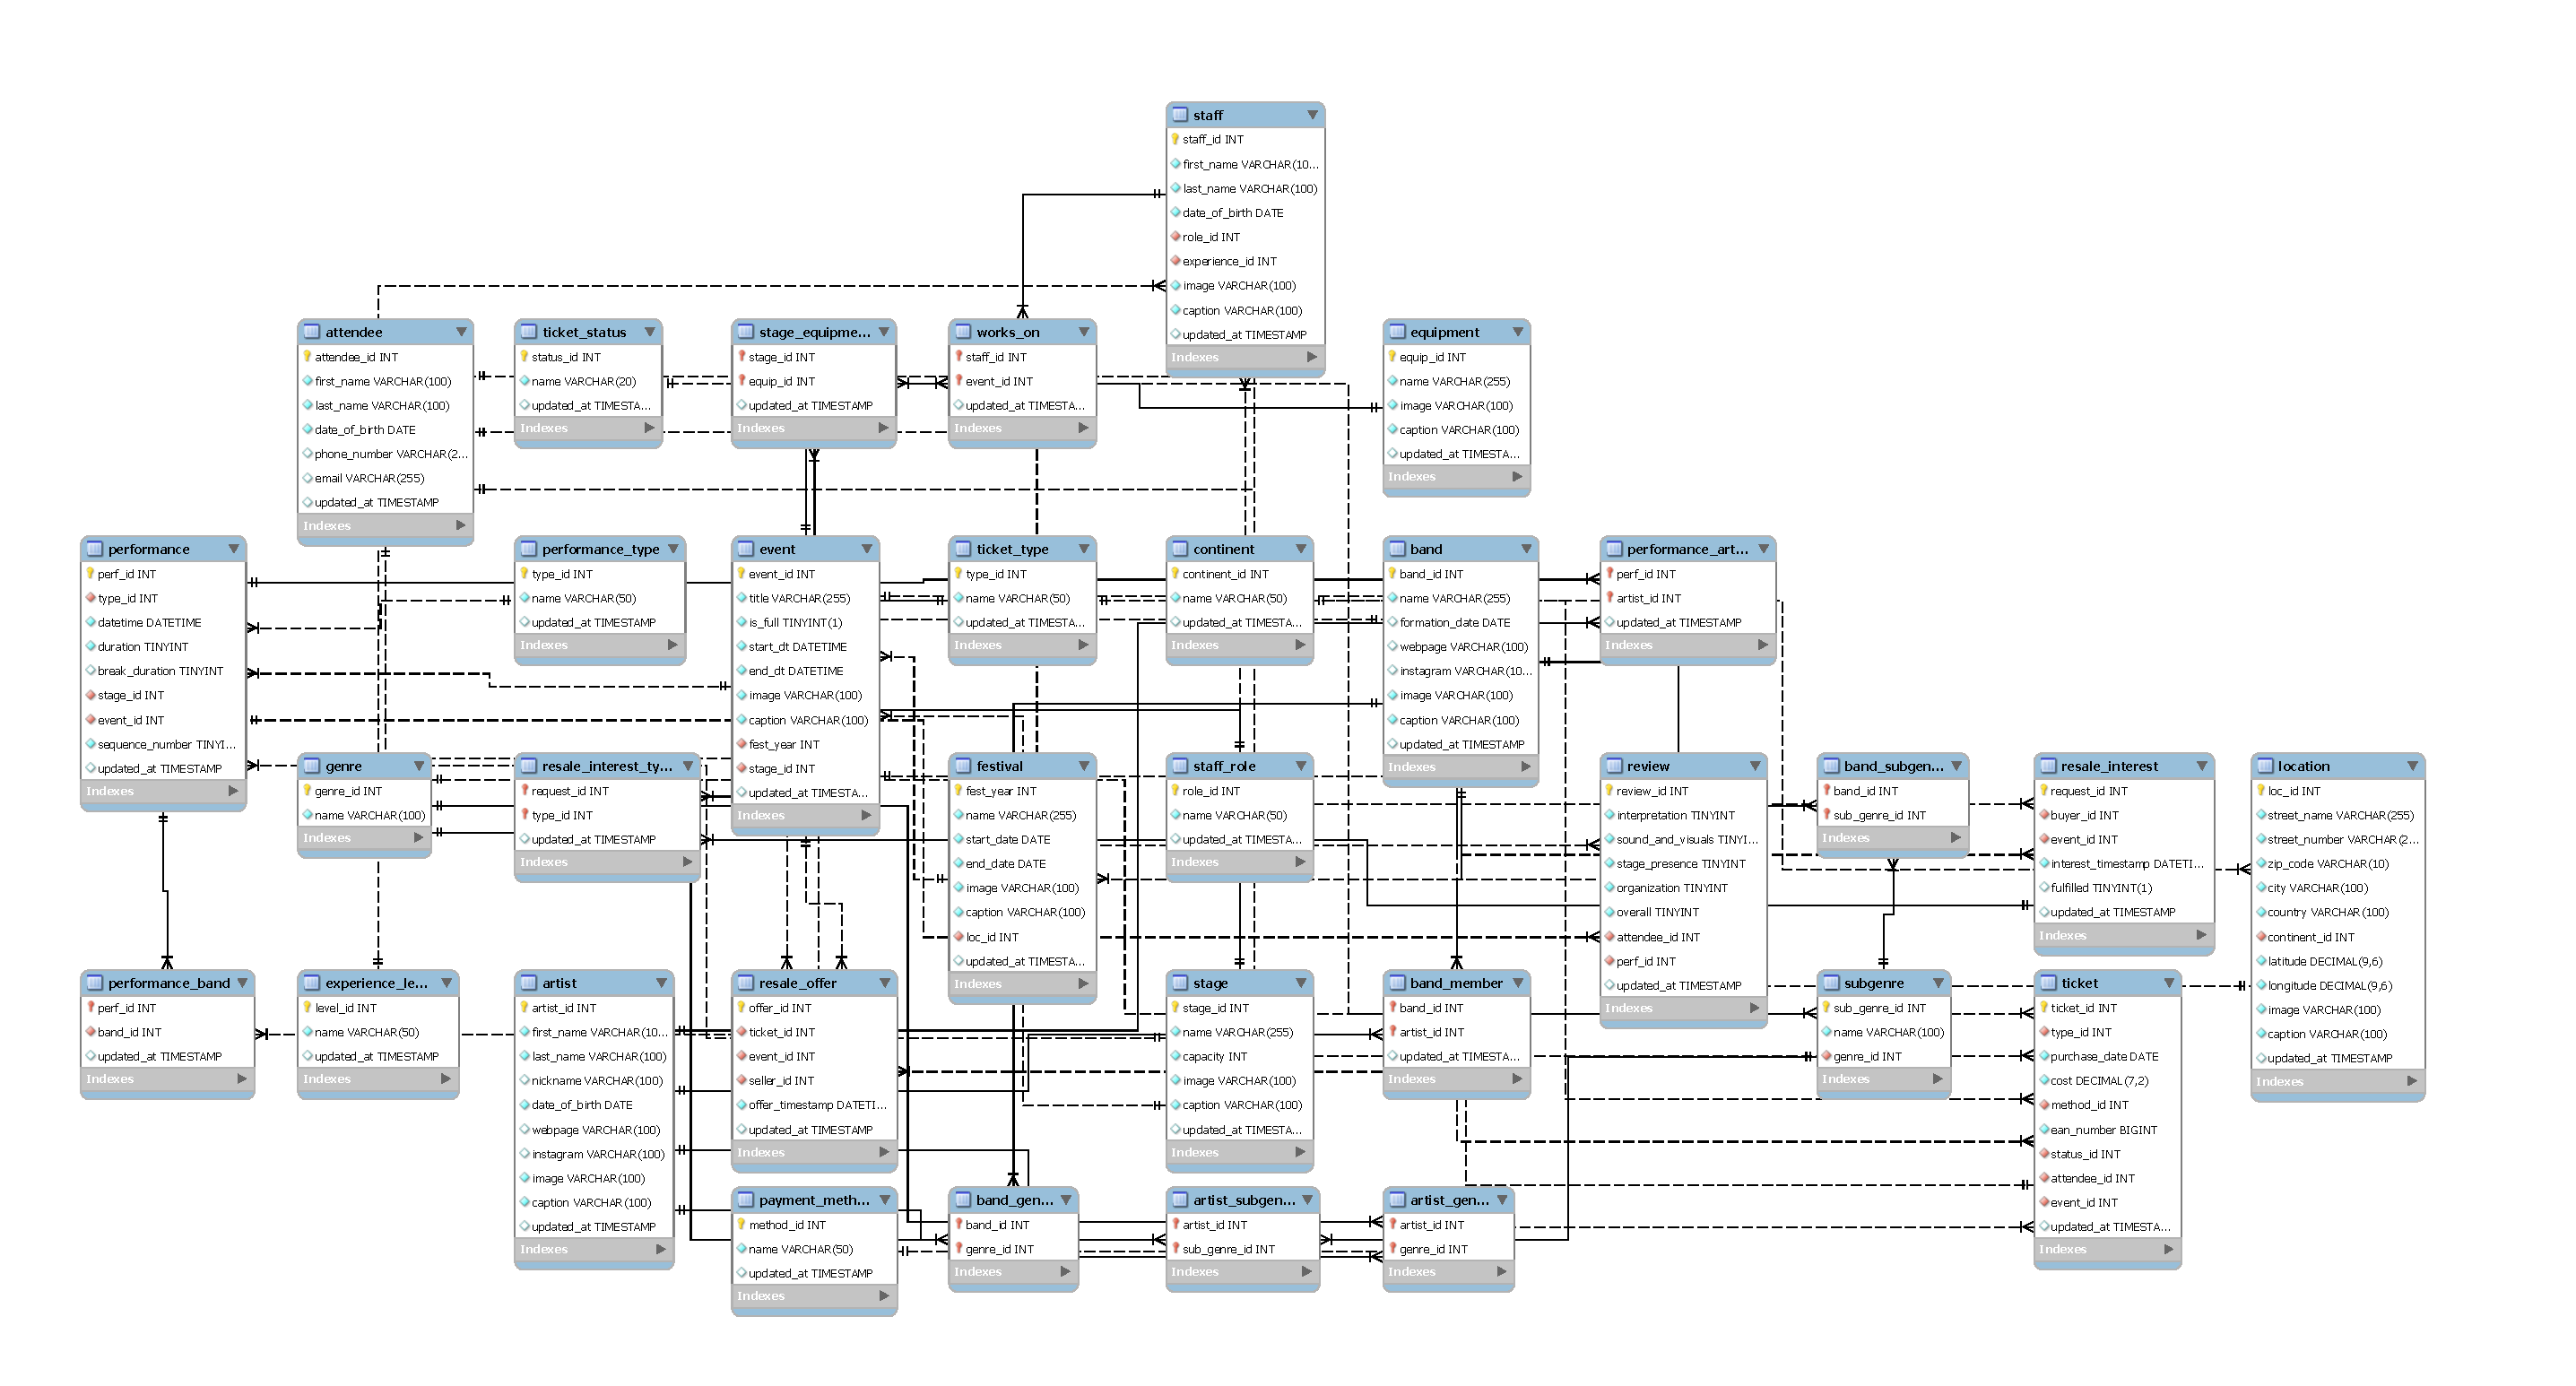
\includegraphics[width=\textwidth]{relational.pdf}
\end{center}
\vspace{5cm}

\subsection{Παραδοχές Υλοποίησης}

Κατά τον σχεδιασμό και την υλοποίηση του συστήματος διαχείρισης δεδομένων για το φεστιβάλ \textit{Pulse University}, ελήφθησαν υπόψη οι προδιαγραφές της εκφώνησης. Παρόλα αυτά, προκειμένου να διασφαλιστεί η πληρότητα και η ορθότητα της βάσης δεδομένων, έγιναν οι ακόλουθες \textbf{παραδοχές υλοποίησης}, οι οποίες δεν καθορίζονται ρητά στην εκφώνηση:

\begin{itemize}
    \item \textbf{Ήπειροι}: Θεωρήθηκε ότι το φεστιβάλ λαμβάνει χώρα κάθε χρόνο σε μία από τις εξής 6 ηπείρους: Αφρική, Ασία, Ευρώπη, Βόρεια Αμερική, Νότια Αμερική, Ωκεανία.

    \item \textbf{Staff Roles}: Θεωρήθηκε ότι κάθε μέλος του προσωπικού λαμβάνει έναν από τους εξής ρόλους: security, support, sound engineer, light technician, stagehand, medic, cleaning, backstage assistant. Όλες οι κατηγορίες πέραν του προσωπικού ασφαλείας (security) και του βοηθητικού προσωπικού (support) θεωρηούνται τεχνικό προσωπικό. Οι περιορισμοί που διατυπώνονται στην εκφώνηση περί security (5\%) και support (2\%) ερμηνεύτηκαν στατικά, ως προς τη χωρητικότητα της κάθε σκηνής, και όχι δυναμικά, ως προς τον πραγματικό αριθμό των θεατών. Δεν θεωρήθηκε επιπλέον απαίτηση του τεχνικού προσωπικού για τη λειτουργία κάθε σκηνής.

    \item \textbf{Κατηγορίες εισιτηρίων}: Όλα τα εισιτήρια ανήκουν σε μία από τις παρακάτω κατηγορίες: general, VIP, backstage, early bird, student. Ο μόνος περιορισμςό που επιβλήθηκε επί αυτών αφορά στα VIP εισιτήρια, τα οποία, σύμφωνα με την εκφώνηση, δεν μπορούν να υπερβαίνουν το 10\% της χωρητικότητας της σκηνής.
    
    \item \textbf{Ημερομηνία αγοράς εισιτηρίου}: Θεωρήθηκε ότι η αγορά του κάθε εισιτηρίου μπορεί να γίνει απαραίτητα την ίδια χρονιά (άρα σίγουρα μετά την ολοκλήρωση του προηγούμνενου φεστιβάλ), και έως τη στιγμή έναρξης της παράστασης στην οποίαν αφορά.
    
    \item \textbf{Αριθμοί EAN13}: Θεωρήθηκαν έγκυροι αριθμοί ΕΑΝ13 μόνο όσοι πληρούν τον έλεγχο του τελευταίου ψηφίου (checksum).

    \item \textbf{Μουσικά είδη}: Έχουμε θεωρήσει 10 μουσικά είδη, και περί τα 3 υποείδη για το κάθε είδος. Τα είδα και τα υποείδη φαίνονται λεπτομερώς στους πίνακες Genre και SubGenre του σχήματος της Βάσης.

    \item \textbf{Καλλιτέχνες και συγκροτήματα}: Όλοι οι μουσικοί, είτε ερμηνεύον σόλο, είτε σε συγκροτήματα, καταχωρούνται στη Βάση ως ξεχωριστοί καλλιτέχνες (Artists). Κάθε συγκρότημα (Band) είναι ένα μοναδικό υποσύνολο του συνόλου των καλλιτεχνών, πληθικότητας τουλάχιστον δύο. Ένας καλλιτέχνης μπορεί να ανήκει σε κανένα ή περισσότερα συγκροτήματα.

    \item \textbf{Μουσικά είδη και συγκροτήματα}: Έχουμε θεωρήσει ότι κάθε καλλιτέχνης χαρακτηρίζεται, πιθανώς μεταξύ άλλων, και από τα μουσικά είδη όλων των συγκροτημάτων στα οποία είναι μέλος. Το αντίστροφο δεν έχει θεωρηθεί.
    
    \item \textbf{Αυτόματη συσχέτιση συγκροτήματος σε εμφάνιση}: Αν όλοι οι καλλιτέχνες μιας εμφάνισης είναι μέλη του ίδιου συγκροτήματος, και δεν υπάρχει άλλο μέλος στο συγκρότημα αυτό, τότε θεωρήθηκε ότι αυτομάτως εμφανίζεται και το ίδιο το συγκρότημα.

    \item \textbf{Παραστάσεις ανά ημέρα}: Έχει θεωρηθεί ότι λαμβάνει χώρα ακριβώς μία παράσταση (event) ανά ημέρα του κάθε φεστιβάλ. Η παραδοχή αυτή προέκυψε από την λογική συναλήθευση των δύο παρακάτω προτάσεων της εκφώνησης: "Κάθε επισκέπτης μπορεί να αγοράσει ένα εισιτήριο ανά ημέρα και παράσταση, αλλά μπορεί να αγοράσει εισιτήρια για κάθε παράσταση και ημέρα του φεστιβάλ."
\end{itemize}


% ─────────────── 3. Υλοποίηση Σχήματος ───────────────
\clearpage
\section{Υλοποίηση Σχήματος}
\subsection{Table Constraints}

Σε αυτήν την ενότητα παρουσιάζουμε τους περιορισμούς ακεραιότητας που επιβάλλονται μαζί με τους ορισμούς των πινάκων, στο αρχείο \texttt{install.sql}. Οι περιορισμοί αυτοί εξασφαλίζουν τη λογική ορθότητα, τη συνέπεια με την εκφώνηση, αλλά και εν γένει την κατά το δυνατόν πιστή αναπαράσταση των πραγματικών συμβάσεων που σχετίζονται με την οργάνωση ενός φεστιβάλ μουσικής.

\subsubsection{Primary Keys}

Για κάθε οντότητα έχει οριστεί πρωτεύον κλειδί, το οποίο εγγυάται τη μοναδικότητα των εγγραφών και τη δυνατότητα αξιόπιστης ταυτοποίησής τους. Οι βασικοί πίνακες, όπως οι \texttt{Artist}, \texttt{Ticket}, \texttt{Stage}, κ.λπ., διαθέτουν απλά πρωτεύοντα κλειδιά (auto-increment IDs). Οι πίνακες που μοντελοποιούν συσχετίσεις many-to-many (π.χ. \texttt{Artist\_Genre}, \texttt{Band\_Member}) χρησιμοποιούν σύνθετα πρωτεύοντα κλειδιά.

Η χρήση των πρωτεύοντων κλειδιών επιτρέπει την ασφαλή συσχέτιση δεδομένων μεταξύ των οντοτήτων και την αποφυγή διπλοεγγραφών.

\subsubsection{Foreign Keys}

Η αναφορική ακεραιότητα επιτυγχάνεται με τη χρήση ξένων κλειδιών που συνδέουν τις οντότητες μεταξύ τους. Κάθε τέτοια σύνδεση διασφαλίζει ότι δεν μπορούν να υπάρξουν εγγραφές που αναφέρονται σε στοιχεία που δεν υπάρχουν στον άμεσα συσχετισμένο πίνακα. Ενδεικτικά παραδείγματα είναι η συσχέτιση των εισιτηρίων με τους επισκέπτες (\texttt{Ticket.attendee\_id}) και των παραστάσεων με τα αντίστοιχα φεστιβάλ (\texttt{Event.fest\_year}).

Όπου η λογική λειτουργίας του φεστιβάλ το απαιτεί, εφαρμόζεται \texttt{ON DELETE CASCADE} για αυτόματο καθαρισμό εξαρτώμενων εγγραφών, ενώ σε κρίσιμα σημεία επιλέγεται \texttt{ON DELETE RESTRICT} για αποτροπή ανεπιθύμητων διαγραφών.

\subsubsection{Unique Constraints}

Για την αποφυγή διπλοτύπων και την εφαρμογή ειδικών κανόνων, έχουν οριστεί περιορισμοί μοναδικότητας (unique constraints) σε συγκεκριμένα πεδία. Χαρακτηριστικά παραδείγματα είναι η μοναδικότητα του ονόματος μιας ηπείρου (\texttt{Continent.name}), του κωδικού EAN13 κάθε εισιτηρίου (\texttt{Ticket.ean\_number}), καθώς και η απαίτηση να μην μπορεί κάποιος επισκέπτης να αγοράσει δεύτερο εισιτήριο για το ίδιο event (\texttt{Ticket.attendee\_id, event\_id}).

Αυτοί οι περιορισμοί αποτρέπουν την ύπαρξη λογικών σφαλμάτων στη βάση δεδομένων και διασφαλίζουν την ορθότητα των δεδομένων σε κρίσιμες περιπτώσεις.

\subsubsection{Check Constraints}

Για την προστασία της ποιότητας των δεδομένων, έχουν οριστεί περιορισμοί ελέγχου (check constraints) σε συγκεκριμένα πεδία. Ενδεικτικά παραδείγματα περιλαμβάνουν:
\begin{itemize}
    \item Εξασφάλιση θετικής τιμής στη χωρητικότητα σκηνής (\texttt{Stage.capacity > 0}).
    \item Έλεγχος ορίων στη διάρκεια εμφανίσεων, ορισμένων από την εκφώνηση (\texttt{Performance.duration BETWEEN 1 AND 180}).
    \item Έλεγχος ότι η αγορά εισιτηρίων γίνεται απαραίτητα πριν την έναρξη του event (\texttt{Ticket.purchase\_date < Event.start\_dt}).
    \item Εξασφάλιση χρήσης έγκυρων URL για εικόνες (\texttt{image LIKE 'https://\%'}).
    \item Ορθό format για Instagram handles (\texttt{instagram LIKE '@\%'}).
\end{itemize}

Οι περιορισμοί αυτοί αποτρέπουν την εισαγωγή μη αποδεκτών τιμών και προστατεύουν από συντακτικά ή λογικά σφάλματα.

\subsubsection{Composite Foreign Keys}

Σε περιπτώσεις όπου απαιτείται η ταυτόχρονη σύνδεση δύο ή περισσότερων πεδίων για τον ορισμό μιας σχέσης, χρησιμοποιούνται σύνθετα ξένα κλειδιά. Ένα χαρακτηριστικό παράδειγμα είναι ο πίνακας \texttt{Performance}, στον οποίο η αναφορά σε event και stage γίνεται μέσω composite foreign key \texttt{(event\_id, stage\_id)}.

Με αυτόν τον τρόπο διασφαλίζεται ότι κάθε εμφάνιση συνδέεται με το σωστό ζεύγος event-stage, αποτρέποντας την ύπαρξη λανθασμένων συνδυασμών.

\subsection{Indexing}

Σε αυτήν την ενότητα παρουσιάζουμε τα ευρετήρια (indexes) που έχουν οριστεί στο αρχείο \texttt{indexing.sql}. Τα ευρετήρια χρησιμοποιούνται για τη βελτίωση της απόδοσης στις αναζητήσεις, στις συνενώσεις (joins) και στους περιορισμούς μοναδικότητας. Ο ορισμός τους είναι κρίσιμος για την αποδοτική εκτέλεση των ερωτημάτων του φεστιβάλ.

\subsubsection{Primary Indexes (Clustered)}

Οι πρωτεύοντες δείκτες δημιουργούνται αυτόματα από τα \texttt{PRIMARY KEY} κάθε πίνακα και διασφαλίζουν τη γρήγορη προσπέλαση των εγγραφών μέσω των πρωτευόντων κλειδιών. Ενδεικτικά:
\begin{itemize}
    \item Ο πίνακας \texttt{Ticket} έχει primary index στο πεδίο \texttt{ticket\_id}.
    \item Ο πίνακας \texttt{Performance} έχει primary index στο \texttt{perf\_id}.
\end{itemize}
Οι primary indexes είναι clustered και επιβάλλουν τη φυσική διάταξη των εγγραφών στον δίσκο, γεγονός που βελτιστοποιεί τις αναζητήσεις μέσω των primary keys.

\subsubsection{Unique Indexes}

Κάθε \texttt{UNIQUE} constraint δημιουργεί αυτόματα ένα μοναδικό ευρετήριο, το οποίο εξασφαλίζει τόσο τη γρήγορη αναζήτηση όσο και την αποτροπή διπλότυπων τιμών. Για παράδειγμα:
\begin{itemize}
    \item Ο πίνακας \texttt{Ticket} έχει unique index στο πεδίο \texttt{ean\_number} (EAN-13 barcode).
    \item Ο πίνακας \texttt{Event} διαθέτει unique index στον συνδυασμό \texttt{(event\_id, stage\_id)}.
\end{itemize}

\subsubsection{Secondary Indexes (Non-Unique)}

Εκτός των primary και unique indexes, έχουν οριστεί και δευτερεύοντα ευρετήρια για τη βελτιστοποίηση ερωτημάτων που βασίζονται σε μη-μοναδικά πεδία.

\paragraph{Χαρακτηριστικά παραδείγματα:}
\begin{itemize}
    \item \texttt{idx\_artist\_dob} στον πίνακα \texttt{Artist}, για ταχύτερη εύρεση καλλιτεχνών βάσει ημερομηνίας γέννησης (χρήσιμο για ερωτήματα ηλικιακής κατάταξης).
    \item \texttt{idx\_event\_start} στον πίνακα \texttt{Event}, που επιταχύνει τα ερωτήματα εύρεσης events βάσει ημερομηνίας έναρξης.
    \item \texttt{idx\_ticket\_attendee\_event} στον πίνακα \texttt{Ticket}, για την ταχεία εύρεση εισιτηρίων ανά επισκέπτη και event.
\end{itemize}
Οι δείκτες αυτοί στοχεύουν στη βελτίωση της απόδοσης σε συχνά εκτελούμενα ερωτήματα και συσχετίσεις.

\subsubsection{Composite Indexes}

Σε περιπτώσεις όπου τα ερωτήματα φιλτράρουν ταυτόχρονα από περισσότερα πεδία, δημιουργούνται σύνθετα ευρετήρια (composite indexes). Ενδεικτικά:
\begin{itemize}
    \item \texttt{idx\_ticket\_event\_date\_payment} στον πίνακα \texttt{Ticket}, που επιταχύνει αναζητήσεις εισιτηρίων βάσει \texttt{event\_id}, \texttt{purchase\_date} και \texttt{method\_id}.
    \item \texttt{idx\_review\_perf\_attendee\_overall} στον πίνακα \texttt{Review}, που διευκολύνει τα ερωτήματα σύγκρισης επιδόσεων καλλιτεχνών ανά επισκέπτη και συνολική αξιολόγηση.
\end{itemize}
Η επιλογή σύνθετων ευρετηρίων γίνεται με βάση τις πραγματικές ανάγκες των ερωτημάτων, όπως αυτές ορίζονται στις προδιαγραφές της εργασίας.

\subsubsection{Index Usage Rationale}

Η επιλογή και τοποθέτηση των indexes βασίζεται σε δύο κριτήρια:
\begin{enumerate}
    \item Την υποστήριξη των ερωτημάτων αξιολόγησης (Q01-Q15), όπως π.χ. η εύρεση ετήσιων εσόδων ανά μέθοδο πληρωμής, οι συμμετοχές καλλιτεχνών και οι αξιολογήσεις.
    \item Την αποδοτικότητα στις συνενώσεις (joins) μεταξύ πινάκων μεγάλου όγκου, όπως \texttt{Ticket}, \texttt{Performance\_Artist}, \texttt{Review}.
\end{enumerate}
Τα indexes μειώνουν δραστικά τον χρόνο αναζήτησης και προσφέρουν βελτιστοποίηση στην εκτέλεση σύνθετων queries, χωρίς να επιβαρύνουν υπερβολικά την εισαγωγή δεδομένων.

\subsection{Triggers}

Σε αυτήν την ενότητα παρουσιάζουμε τους περιορισμούς ακεραιότητας που υλοποιούνται μέσω triggers, όπως ορίζονται στο αρχείο \texttt{Triggers.sql}. Οι περιορισμοί αυτοί επιβάλλουν πιο σύνθετους κανόνες που δεν μπορούν να εκφραστούν απευθείας μέσω constraints στους πίνακες και εξασφαλίζουν τη δυναμική συνέπεια των δεδομένων, βάσει των λογικών απαιτήσεων του φεστιβάλ.

\subsubsection{Participation Rules}

Triggers αυτής της κατηγορίας επιβάλλουν κανόνες συμμετοχής καλλιτεχνών και συγκροτημάτων σε εμφανίσεις (performances).

\begin{itemize}
    \item \textbf{Performance Band Validation} (\texttt{trg\_band\_validate\_before\_ins}): Ελέγχει ότι δεν γίνεται ανάθεση δεύτερου συγκροτήματος στην ίδια εμφάνιση και ότι οι ήδη ανατεθειμένοι καλλιτέχνες είναι μέλη του συγκροτήματος.
    \item \textbf{Performance Artist Validation} (\texttt{trg\_artist\_validate\_before\_ins}): Ελέγχει ότι όταν υπάρχει ήδη συσχετισμένο συγκρότημα, ο νέος καλλιτέχνης είναι υποχρεωτικά μέλος του. Επίσης, αν δεν υπάρχει συγκρότημα, επιβάλλει κοινή συμμετοχή σε συγκρότημα μεταξύ των καλλιτεχνών.
    \item \textbf{Auto-Band Assignment} (\texttt{trg\_auto\_assign\_band\_after\_artist\_ins}): Όταν όλοι οι καλλιτέχνες μιας εμφάνισης ανήκουν στο ίδιο συγκρότημα, αυτό προστίθεται αυτόματα στην Performance.
\end{itemize}

Οι triggers αυτοί εξασφαλίζουν ότι η συσχέτιση καλλιτεχνών και συγκροτημάτων γίνεται με συνέπεια και ότι δεν δημιουργούνται λανθασμένες ή ασυνεπείς αναθέσεις.

\subsubsection{Scheduling Constraints}

Αυτή η κατηγορία triggers ελέγχει κανόνες προγραμματισμού (scheduling) και χρονικής τοποθέτησης.

\begin{itemize}
    \item \textbf{No Double Stage Artist} (\texttt{trg\_no\_double\_stage\_artist}): Αποτρέπει την ανάθεση καλλιτέχνη σε δύο σκηνές την ίδια χρονική στιγμή.
    \item \textbf{No Double Stage Band} (\texttt{trg\_no\_double\_stage\_band}): Αντίστοιχος έλεγχος για συγκροτήματα.
    \item \textbf{No Stage Overlap} (\texttt{trg\_no\_stage\_overlap}): Διασφαλίζει ότι δεν προγραμματίζεται δεύτερη εμφάνιση σε σκηνή όταν υπάρχει χρονική επικάλυψη.
    \item \textbf{Max Consecutive Years} (\texttt{trg\_max\_consecutive\_years\_artist}, \texttt{trg\_max\_consecutive\_years\_band}): Επιβάλλουν τον περιορισμό συμμετοχής έως 3 συνεχόμενα έτη.
    \item \textbf{Event Within Festival} (\texttt{trg\_event\_within\_festival\_dates}): Ελέγχει ότι οι ημερομηνίες των events εμπίπτουν στα όρια του φεστιβάλ.
    \item \textbf{Performance Inside Event} (\texttt{trg\_performance\_inside\_event}): Διασφαλίζει ότι η εμφάνιση εκτελείται εντός του χρονικού πλαισίου του event.
\end{itemize}

Οι triggers αυτοί αποτρέπουν ασυμβατότητες σε επίπεδο προγράμματος και εξασφαλίζουν τη ρεαλιστική λειτουργία του φεστιβάλ.

\subsubsection{Data Safety and Cleanup}

Triggers που προστατεύουν την ακεραιότητα των δεδομένων κατά την ενημέρωση ή διαγραφή εγγραφών.

\begin{itemize}
    \item \textbf{Safe Date Updates} (\texttt{trg\_safe\_festival\_date\_update}, \texttt{trg\_safe\_event\_date\_update}): Ελέγχουν ότι η τροποποίηση ημερομηνιών φεστιβάλ ή event δεν παραβιάζει ήδη προγραμματισμένες εμφανίσεις.
    \item \textbf{Band Auto-Deletion} (\texttt{trg\_delete\_band\_if\_no\_members}): Διαγράφει αυτόματα συγκρότημα όταν δεν έχει πια μέλη.
    \item \textbf{Cascade Cleanup for Attendee} (\texttt{trg\_delete\_attendee\_cleanup}): Με την διαγραφή ενός επισκέπτη, διαγράφονται τα εισιτήρια, οι προσφορές, τα ενδιαφέροντα και οι αξιολογήσεις του.
\end{itemize}

Με αυτά τα triggers, προστατεύεται η συνοχή των δεδομένων σε περιπτώσεις τροποποίησης ή διαγραφής, αποφεύγοντας ασυνεπή ή "ορφανά" δεδομένα.

\subsubsection{Ticketing Rules}

Triggers που διασφαλίζουν την ορθή διαχείριση των εισιτηρίων.

\begin{itemize}
    \item \textbf{Capacity Control} (\texttt{trg\_ticket\_capacity\_check}): Αποτρέπει την υπέρβαση της χωρητικότητας σκηνής.
    \item \textbf{VIP Ticket Limit} (\texttt{trg\_check\_vip\_ticket\_limit}): Ελέγχει ότι τα VIP εισιτήρια δεν υπερβαίνουν το 10\% της χωρητικότητας.
    \item \textbf{EAN Validation} (\texttt{trg\_validate\_ticket\_ean}, \texttt{trg\_validate\_ticket\_ean\_upd}): Υλοποιούν έλεγχο εγκυρότητας του EAN-13 checksum κατά την εισαγωγή ή τροποποίηση εισιτηρίων.
    \item \textbf{Immutable Purchase Date} (\texttt{trg\_block\_purchase\_date\_update}): Αποτρέπει την αλλαγή της ημερομηνίας αγοράς μετά την εισαγωγή.
    \item \textbf{Purchase Deadline} (\texttt{trg\_validate\_ticket\_purchase\_date}): Ελέγχει ότι τα εισιτήρια αγοράζονται πριν την έναρξη του event.
\end{itemize}

Αυτοί οι triggers εγγυώνται την αξιοπιστία της διαδικασίας έκδοσης και διαχείρισης εισιτηρίων, ευθυγραμμισμένα με τους κανόνες του φεστιβάλ.

\subsubsection{Resale and Reviews}

Triggers που σχετίζονται με τη λειτουργία μεταπώλησης εισιτηρίων και την αξιολόγηση εμφανίσεων.

\begin{itemize}
    \item \textbf{Resale Eligibility} (\texttt{trg\_resale\_offer\_only\_active}): Επιτρέπει μεταπώληση μόνο για ενεργά εισιτήρια.
    \item \textbf{Review Eligibility} (\texttt{trg\_review\_only\_with\_used\_ticket}): Επιτρέπει αξιολόγηση μόνο εφόσον έχει χρησιμοποιηθεί εισιτήριο.
    \item \textbf{Immutable Timestamps} (\texttt{trg\_resale\_offer\_timestamp}, \texttt{trg\_resale\_interest\_timestamp}): Αποτρέπουν την αλλοίωση timestamps σε προσφορές και ενδιαφέροντα.
    \item \textbf{Automatic Matching} (\texttt{trg\_match\_resale\_interest}, \texttt{trg\_match\_resale\_offer}): Υλοποιούν αυτόματη αντιστοίχιση αγοραστών και πωλητών σε ουρά FIFO.
\end{itemize}

Αυτοί οι triggers εξασφαλίζουν την εύρυθμη λειτουργία της αγοράς μεταπώλησης και την ορθότητα των αξιολογήσεων.

\subsubsection{Operational Rules}

\begin{itemize}
    \item \textbf{Staff Ratio Enforcement} (\texttt{trg\_staff\_ratio\_after\_delete}, \texttt{trg\_staff\_ratio\_after\_update}): Ελέγχουν ότι η αναλογία ασφαλείας (5\%) και υποστήριξης (2\%) παραμένει εντός ορίων μετά από αλλαγές στον προγραμματισμό προσωπικού.
    \item \textbf{Stage Capacity Adjustments} (\texttt{trg\_stage\_capacity\_update}): Αποτρέπει τη μείωση χωρητικότητας σκηνής και επανενεργοποιεί events ως \texttt{is\_full = FALSE} σε περίπτωση αύξησης.
    \item \textbf{Event Date Generation} (\texttt{trg\_set\_event\_date}): Θέτει αυτόματα το \texttt{generated\_date} από την ημερομηνία έναρξης του event.
\end{itemize}

Αυτά τα triggers υποστηρίζουν τη σωστή λειτουργία των επιχειρησιακών διαδικασιών του φεστιβάλ, πέραν της απλής ακεραιότητας.

\subsection{Procedures}

Η βάση δεδομένων \textit{Pulse University} υλοποιεί σειρά αποθηκευμένων διαδικασιών (procedures) για την εφαρμογή κανόνων ακεραιότητας, συντήρησης δεδομένων και λειτουργικών ελέγχων. Κάθε procedure αναφέρεται αναλυτικά παρακάτω:

\subsubsection{UpdateExpiredTickets()}

Η διαδικασία αυτή ενημερώνει την κατάσταση των εισιτηρίων (tickets) σε \texttt{unused} για όλα τα events που έχουν ολοκληρωθεί (η σημερινή ημερομηνία είναι μεταγενέστερη του \texttt{end\_dt} του event). 
\begin{itemize}
    \item Επηρεάζονται μόνο τα εισιτήρια με κατάσταση \texttt{active} ή \texttt{on offer}.
    \item Αποσκοπεί στην αυτόματη ενημέρωση εισιτηρίων που έμειναν αχρησιμοποίητα μετά το τέλος του event.
\end{itemize}

\subsubsection{ExpireResaleOffers()}

Αυτή η procedure διαγράφει όλες τις ενεργές προσφορές μεταπώλησης εισιτηρίων (\texttt{Resale\_Offer}) που σχετίζονται με events τα οποία έχουν ήδη ολοκληρωθεί.
\begin{itemize}
    \item Βασίζεται σε JOIN με τον πίνακα \texttt{Event} για τον έλεγχο ημερομηνιών.
    \item Αποτρέπει την ύπαρξη λανθασμένων ή ανενεργών προσφορών στο σύστημα.
\end{itemize}

\subsubsection{ExpireResaleInterests()}

Αντίστοιχη με την προηγούμενη, διαγράφει τα \texttt{Resale\_Interests} (αιτήματα αγοράς) που σχετίζονται με ολοκληρωμένα events.
\begin{itemize}
    \item Εξυπηρετεί τον καθαρισμό της βάσης από αιτήματα που πλέον δεν έχουν νόημα.
\end{itemize}

\subsubsection{ScanTicket(IN p\_ean BIGINT)}

Η procedure αυτή προσομοιώνει τη σάρωση ενός εισιτηρίου στην είσοδο ενός event:
\begin{itemize}
    \item Δέχεται ως παράμετρο τον \texttt{ean\_number} του εισιτηρίου.
    \item Ελέγχει αν το εισιτήριο υπάρχει και αν είναι σε \texttt{active} κατάσταση.
    \item Αν είναι έγκυρο, ενημερώνει την κατάστασή του σε \texttt{used}.
    \item Αν δεν είναι έγκυρο, επιστρέφει αντίστοιχο σφάλμα.
\end{itemize}

\subsubsection{RunMaintenance()}

Πρόκειται για κεντρική διαδικασία συντήρησης που εκτελεί:
\begin{enumerate}
    \item Την ανανέωση καταστάσεων εισιτηρίων (\texttt{UpdateExpiredTickets}).
    \item Τη διαγραφή ληγμένων προσφορών/αιτημάτων (\texttt{ExpireResaleOffers}, \texttt{ExpireResaleInterests}).
    \item Τον έλεγχο στελέχωσης (\texttt{check\_staff\_ratio}) για κάθε event με χρήση cursor.
    \item Χειρίζεται σφάλματα ratio check με warnings ανά event.
\end{enumerate}
Αυτοματοποιεί τις βασικές ενέργειες συντήρησης του φεστιβάλ.

\subsubsection{sp\_rename\_self(IN new\_name VARCHAR(64))}

Αυτή η procedure επιτρέπει στον συνδεδεμένο χρήστη να αλλάξει το username του:
\begin{itemize}
    \item Εντοπίζει το username του caller μέσω της συνάρτησης \texttt{USER()}.
    \item Εκτελεί δυναμικό SQL \texttt{ALTER USER ... RENAME TO} για τη μετονομασία.
    \item Υλοποιείται με \texttt{SQL SECURITY DEFINER} για ελεγχόμενη πρόσβαση.
\end{itemize}
Αφορά λειτουργία ειδικού ενδιαφέροντος για διαχείριση χρηστών.

\subsubsection{check\_staff\_ratio(IN ev INT)}

Η συγκεκριμένη procedure ελέγχει αν η στελέχωση ενός event πληροί τις ελάχιστες απαιτήσεις:
\begin{itemize}
    \item Τουλάχιστον 5\% της χωρητικότητας της σκηνής σε \texttt{security staff}.
    \item Τουλάχιστον 2\% της χωρητικότητας σε \texttt{support staff}.
\end{itemize}
Σε περίπτωση παραβίασης, επιστρέφει σφάλμα SQLSTATE '45000'.  
Χρησιμοποιείται και αυτόνομα, αλλά και μέσα από το \texttt{RunMaintenance()}.

\vspace{0.5cm}
Η υλοποίηση αυτών των procedures καλύπτει βασικούς άξονες λειτουργικότητας: συντήρηση δεδομένων, επιχειρησιακοί έλεγχοι, προσομοίωση χρήσης (ticket scanning), και διαχείριση χρηστών, συνεισφέροντας στη συνοχή και αξιοπιστία της βάσης δεδομένων.


\subsection{Views}

Η υλοποίηση του συστήματος \textit{Pulse University} περιλαμβάνει σειρά από views, τα οποία χρησιμοποιούνται τόσο για την απλοποίηση πολύπλοκων ερωτημάτων, όσο και για τη βελτίωση της αναγνωσιμότητας και της απόδοσης. Κάθε view εξυπηρετεί συγκεκριμένο επιχειρησιακό στόχο, όπως αναλύεται παρακάτω.

\subsubsection{View\_Yearly\_Revenue\_By\_Method}

Το view αυτό συγκεντρώνει τα συνολικά έσοδα από πωλήσεις εισιτηρίων, ομαδοποιημένα ανά έτος διεξαγωγής φεστιβάλ (\texttt{fest\_year}) και μέθοδο πληρωμής (\texttt{method\_id}).

\begin{itemize}
    \item Εξάγει άμεσα τα δεδομένα για το ερώτημα Q01 (Yearly Revenues by Payment Method).
    \item Υπολογίζει \texttt{SUM(t.cost)} πάνω στον πίνακα \texttt{Ticket}, συνενώνοντας με \texttt{Event} για να εντοπίσει το αντίστοιχο \texttt{fest\_year}.
\end{itemize}

\subsubsection{View\_Artist\_Year\_Participation}

Το view αυτό παρέχει λίστα με καλλιτέχνες και τα έτη στα οποία συμμετείχαν σε φεστιβάλ.

\begin{itemize}
    \item Χρησιμοποιείται στο ερώτημα Q02 (αν συμμετείχαν σε συγκεκριμένο έτος).
    \item Συνδέει τους πίνακες \texttt{Performance\_Artist}, \texttt{Performance} και \texttt{Event} για την εξαγωγή του έτους συμμετοχής.
\end{itemize}

\subsubsection{View\_Performance\_Detail}

Παρέχει λεπτομέρειες για κάθε εμφάνιση (performance), συνδυάζοντας:
\begin{itemize}
    \item ID εμφάνισης, event, έτος φεστιβάλ, τύπο εμφάνισης, ημερομηνία.
    \item Πληροφορίες για τον καλλιτέχνη ή συγκρότημα.
\end{itemize}
Είναι χρήσιμο για ερωτήματα όπως το Q03 (π.χ. ζεύγη artist-performance με όλα τα context).

\subsubsection{View\_Artist\_Performance\_Rating}

Υπολογίζει στατιστικά ανά καλλιτέχνη:
\begin{itemize}
    \item Σύνολο εμφανίσεων (\texttt{performance\_count}).
    \item Μέσος όρος βαθμολογίας για \texttt{interpretation} και \texttt{overall}.
\end{itemize}
Απαιτείται στα ερωτήματα Q04 (average interpretation) και Q11 (συγκρίσεις συμμετοχών).

\subsubsection{View\_Attendee\_Event\_Rating}

Συσχετίζει επισκέπτες με events που παρακολούθησαν και υπολογίζει τον μέσο όρο βαθμολογίας που έδωσαν.
\begin{itemize}
    \item Βασίζεται στο \texttt{Ticket}, \texttt{Review} και \texttt{Performance}.
    \item Απαιτείται στο ερώτημα Q06 (average rating per attendee per event).
\end{itemize}

\subsubsection{View\_Attendee\_Yearly\_Visits}

Παρουσιάζει πόσες παραστάσεις παρακολούθησε κάθε επισκέπτης ανά έτος.
\begin{itemize}
    \item Υπολογίζει \texttt{events\_attended} ανά έτος (\texttt{YEAR(purchase\_date)}).
    \item Χρησιμοποιείται στο Q09 (επισκέπτες με περισσότερες από 3 συμμετοχές ανά έτος).
\end{itemize}

\subsubsection{View\_Genre\_Pairs}

Παρέχει τα ζεύγη ειδών μουσικής (genres) που καλύπτονται από τους ίδιους καλλιτέχνες.
\begin{itemize}
    \item Υπολογίζει για καλλιτέχνες που έχουν ήδη εμφανιστεί.
    \item Αφορά το ερώτημα Q10 (top-3 genre pairs με κοινές εμφανίσεις).
\end{itemize}

\subsubsection{View\_Artist\_Continents}

Δείχνει σε πόσες διαφορετικές ηπείρους έχει εμφανιστεί κάθε καλλιτέχνης.
\begin{itemize}
    \item Συσχετίζει καλλιτέχνες με locations μέσω \texttt{Festival} και \texttt{Event}.
    \item Αφορά το ερώτημα Q13 (καλλιτέχνες με παρουσία σε ≥3 ηπείρους).
\end{itemize}

\subsubsection{View\_Genre\_Year\_Counts}

Επιστρέφει τον αριθμό εμφανίσεων ανά είδος μουσικής (genre) και έτος.
\begin{itemize}
    \item Συνδυάζει \texttt{Performance\_Detail} και \texttt{Artist\_Genre}.
    \item Χρήσιμο για το Q14 (συνεχόμενες χρονιές με ίδιο πλήθος εμφανίσεων).
\end{itemize}

\subsubsection{View\_Attendee\_Artist\_Review}

Υπολογίζει τη συνολική βαθμολογία που έχει δώσει κάθε επισκέπτης σε κάθε καλλιτέχνη.
\begin{itemize}
    \item Βασίζεται στη σύνδεση \texttt{Review} και \texttt{Performance\_Artist}.
    \item Απαιτείται για το ερώτημα Q15 (top-5 επισκέπτες με υψηλότερες συνολικές αξιολογήσεις ανά καλλιτέχνη).
\end{itemize}

\vspace{0.5cm}
Τα παραπάνω views σχεδιάστηκαν με σκοπό να απλοποιήσουν την εκτέλεση των σύνθετων ερωτημάτων αξιολόγησης (Q01–Q15), να βελτιώσουν την αναγνωσιμότητα του κώδικα και να μειώσουν τον υπολογιστικό φόρτο μέσω προϋπολογισμένων αποτελεσμάτων.

% ─────────────── 4. Πληθυσμός Δεδομένων ───────────────
\clearpage
\section{Παραγωγή Συνθετικών Δεδομένων}

\subsection{Η Διαδικασία της Παραγωγής}

Η παραγωγή των συνθετικών δεδομένων υλοποιήθηκε με δύο scripts, γραμμένα σε Python:
\begin{itemize}
    \item \texttt{faker.py}, το οποίο παράγει τα δεδομένα και κατόπιν εκτελεί εισαγωγές απευθείας στη βάση δεδομένων, μέσω της MySQL, χρησιμοποιώντας το \texttt{mysql-connector}.
    \item \texttt{faker\_sql.py}, το οποίο παράγει τα δεδομένα και τις αντίστοιχες εντολές SQL και κατόπιν τις γράφει στο αρχείο \texttt{sql/load.sql}, χωρίς ωστόσο να εκτελεί άμεση εισαγωγή στη βάση.
\end{itemize}

Και τα δύο σενάρια σέβονται:
\begin{itemize}
    \item τους \textbf{περιορισμούς ακεραιότητας}, όπως αυτοί ορίζονται στο \texttt{install.sql}, δηλαδή τα foreign keys και τυχόν \texttt{CHECK}, \texttt{NOT NULL}, \texttt{UNIQUE} constraints, κ.τ.ό.
    \item τα \textbf{triggers}, όπως αυτά ορίζονται στο \texttt{triggers.sql}
\end{itemize}
Επιπλέον, παράγουν και καταχωρούν τα δεδομένα σε ειδική σειρά, η οποία προλαμβάνει τυχόν παραβιάσεις κατά την αναφορά στα αντίστοιχα - έως τότε κενά - πεδία ή αλυσιδωτές εξαρτήσεις, ενώ αμφότερα εκτελούν δοκιμαστικά και δειγματοληπτικά queries απεθείας στη βάση, ώστε να επιτευχθεί η επιτυχής εγγραφή νέων δεδομένων, σύμφωνα με τους αντίστοιχους περιορισμούς.

\subsubsection{Εισαγωγή Δεδομένων με \texttt{faker.py}}

Το αρχείο \texttt{faker.py} παράγει συνθετικά δεδομένα και τα εισάγει απευθείας στη βάση δεδομένων, χρησιμοποιώντας το \texttt{mysql-connector} της Python. Η παραγωγή και εισαγωγή των δεδομένων γίνονται σειριακά, ως εξής:
\begin{enumerate}
    \item \textbf{Σταθερές οντότητες:} εξοπλισμός, 36 σκηνές (3 ανά έτος), τοποθεσίες (όσες δεν περιλαμβάνονται στα lookup tables, όπως πόλεις και οδοί), 12 φεστιβάλ (σε χρονολογίες 2016-2027, 2 μελλοντικά) και 4-6 events ανά φεστιβάλ, τα οποία όλα τηρούν τους επιβαλλόμενους από τα triggers περιορισμούς, όπως:
    \begin{itemize}
        \item ένα φεστιβάλ ανά έτος και καταχώρηση δύο μελλοντικών φεστιβάλ, με την παραδοχή ότι το φεστιβάλ του 2025 (φετινό) έχει ήδη ολοκληρωθεί,
        \item τα events εντάσσονται εντός της διάρκειας του φεστιβάλ, θεωρώντας ως ημερομηνία του event την ημέρα έναρξής του.
    \end{itemize}
    \item \textbf{Προσωπικό:} προσωπικό ασφαλείας, προσωπικό υποστήριξης και τεχνικό προσωπικό, με κατανομή βάσει της χωρητικότητας της εκάστοτε σκηνής και χρήση του procedure \texttt{check\_staff\_ratio()} και σεβόμενοι περιορισμούς, όπως:
    \begin{itemize}
        \item επάρκεια βοηθητικού προσωπικού και προσωπικού ασφαλείας, ως συνάρτηση της χωρητικότητας της εκάστοτε σκηνής,
        \item την παραδοχή ότι το προσωπικό εργάζεται μόνο την ημέρα έναρξης του event (σε περίπτωση που αυτό καλύπτει δύο ημέρες, πριν και μετά τις 00:00).
    \end{itemize}
    \item \textbf{Καλλιτέχνες και μπάντες:} 45 καλλιτέχνες και 10 μπάντες με genres και αντίστοιχα subgenres, τηρώντας constraints που επιβάλλονται από τα triggers, όπως:
    \begin{itemize}
        \item αμοιβαίος αποκλεισμός solo artists και bands,
        \item εισαγωγή νέου καλλιτέχνη σε εμφάνιση, μόνο εάν μοιράζεται κοινή μπάντα με όλους όσους έχουν ήδη ανατεθεί στην εμφάνιση αυτή,
        \item η μέγιστη συνεχόμενη συμμετοχή ενός καλλιτέχνη (μέσω μπάντας ή solo) είναι 3 έτη,
        \item δεν επιτρέπεται ταυτόχρονη εμφάνιση σε πολλαπλές σκηνές,
        \item συμβατότητα του subgenre με το genre στο οποίο ανήκει,
        \item και όσα ακόμα αναφέρονται στις αντίστοιχες ενότητες του \texttt{triggers.sql}.
    \end{itemize}
    \clearpage
    \item \textbf{Παραστάσεις:} περιλαμβάνονται 3–6 ανά event, με κατανομή 80\% μπάντες και 20\% solo, και καθορισμένα slots για ``warm up'', ``headline'', κ.τ.ό., σεβόμενες τους περιορισμούς που επιβάλλονται από τα triggers, όπως:
    \begin{itemize}
        \item να βρίσκονται εντός της διάρκειας του event στο οποίο εντάσσονται,
        \item να μην επικαλύπτονται,
        \item να τηρούνται πιστά οι επιτρεπτοί χρόνοι διαλείμματος.
    \end{itemize}
    \item \textbf{Συμμετέχοντες, Εισιτήρια και Κριτικές:} εισαγωγή εισιτηρίων:
    \begin{itemize}
        \item με έγκυρο EAN-13,
        \item ημερομηνία αγοράς πριν την έναρξη του event,
        \item status (\texttt{active}, \texttt{used}, \texttt{on offer} κ.λπ.) ανάλογα με την ημερομηνία του event στο οποίο αναφέρονται (παρελθοντικό ή μελλοντικό),
    \end{itemize}
    ενώ οι κριτικές του performance πρέπει να συνοδεύονται από attendee με used ticket για το συγκεκριμένο event.
    \item \textbf{Ουρά μεταπώλησης:} η ουρά μεταπώλησης λειτουργεί ορθά και από την πλευρά του αγοραστή και από αυτη του πωλητή, μέσω triggers, και καταγράφεται σε log (το οποίο φαίνεται με την εκτέλεση της εντολής \texttt{db137 viewq}), ενώ τα timestamps στα resale entries παραμένουν αμετάβλητα, για λόγους ακεραιότητας.
\end{enumerate}

Η εισαγωγή τερματίζει με αυτόματη (εσωτερική) εκτέλεση του \texttt{db137 db-status} και αποθήκευση του πλήθους των εγγραφών ανά πίνακα στο \texttt{docs/organization/db\_data.txt}.

\subsubsection{Παραγωγή SQL με \texttt{faker\_sql.py}}

Το \texttt{faker\_sql.py} εκτελεί παραγωγή συνθετικών δεδομένων με την ίδια λογική με το \texttt{faker.py}, αλλά καταγράφει τις εντολές SQL που προκύπτουν στο αρχείο \texttt{sql/load.sql}, το οποίο:
\begin{itemize}
    \item μπορεί να εκτελεστεί ανεξάρτητα, σε οποιοδήποτε περιβάλλον, για λόγους αναπαραγωγής των δεδομένων (τα οποία παράγονται πιθανοτικά) και των αποτελεσμάτων των ερωτημάτων,
    \item ενσωματώνεται στο CLI μέσω της εντολής \texttt{load-db --g}, όπου και εκτελείται, γράφει στο αρχείο load.sql και κατόπιν φορτώνει τα δεδομένα του στη βάση.
\end{itemize}

Η έξοδος του query στο \texttt{load.sql} παράγεται μόνο αν κάθε \texttt{INSERT} ολοκληρωθεί επιτυχώς. Αν υπάρξει παραβίαση σε επίπεδο entity ή trigger, τότε η εγγραφή παραλείπεται.

\subsection{Εξασφάλιση Κάλυψης Ερωτημάτων}

Για να διασφαλιστεί η επιτυχής εκτέλεση και η επιστροφή επαρκών και αντιπροσωπευτικών δεδομένων σε όλα τα ερωτήματα (Q01 -- Q15), ενσωματώθηκαν ρητές δομές δεδομένων, στην ενότητα 8 των αρχείων \texttt{faker.py} και \texttt{faker\_sql.py}. Ειδικότερα, μεριμνήσαμε για τα εξής:
\begin{itemize}
    \item \textbf{Q1:} Καθορίζεται ηλικιακή κατανομή στους καλλιτέχνες: 65\% κάτω των 30 ετών.
    \item \textbf{Q3:} Για κάθε έτος υπάρχουν τουλάχιστον 3 εμφανίσεις τύπου ``warm up''.
    \item \textbf{Q5:} Έξι καλλιτέχνες κάτω των 30 εξισώνονται σε αριθμό εμφανίσεων με τον πρώτο σε εμφανίσεις, μέσω επιπλέον εμφανίσεων ή νέων bands.
    \item \textbf{Q9:} 50 attendees έχουν 4 ή περισσότερα εισιτήρια στο ίδιο έτος
    \item \textbf{Q11:} Οι attendees \#1 και \#2 αξιολογούν από κοινού τουλάχιστον 5 εμφανίσεις του ίδιου artist.
    \item \textbf{Q14:} Εμφανίζονται τουλάχιστον 3 εμφανίσεις Rock, Pop και Jazz για καθένα από τα έτη 2024 και 2025.
\end{itemize}

\clearpage
\subsection{Τα Δεδομένα της Βάσης}

Ο παρακάτω πίνακας παρουσιάζει το πλήθος εγγραφών ανά πίνακα της βάσης δεδομένων, μετά την εκτέλεση του \texttt{faker\_sql.py} και την εισαγωγή των δεδομένων από το \texttt{load.sql}. Η αποτύπωση πραγματοποιείται αυτόματα μέσω της εντολής \texttt{db137 db-status} και αποθηκεύεται στο αρχείο \texttt{db\_data.txt}.

\vspace{1cm}
\begin{center}
\begin{tabular}{|l|r|}
\hline
\textbf{Πίνακας} & \textbf{Πλήθος Εγγραφών} \\
\hline
Artist & 55 \\
Artist\_Genre & 100 \\
Artist\_SubGenre & 100 \\
Attendee & 2000 \\
Band & 10 \\
Band\_Genre & 20 \\
Band\_Member & 29 \\
Band\_SubGenre & 20 \\
Continent & 6 \\
Equipment & 30 \\
Event & 58 \\
Experience\_Level & 5 \\
Festival & 12 \\
Genre & 10 \\
Location & 12 \\
Payment\_Method & 3 \\
Performance & 260 \\
Performance\_Artist & 426 \\
Performance\_Band & 158 \\
Performance\_Type & 5 \\
Resale\_Interest & 20 \\
Resale\_Interest\_Type & 20 \\
Resale\_Match\_Log & 80 \\
Resale\_Offer & 70 \\
Review & 9733 \\
Staff & 60 \\
Staff\_Role & 8 \\
Stage & 36 \\
Stage\_Equipment & 263 \\
SubGenre & 30 \\
Ticket & 5536 \\
Ticket\_Status & 4 \\
Ticket\_Type & 5 \\
Works\_On & 788 \\
\hline
\end{tabular}
\end{center}


% ─────────────── 5. Τεκμηρίωση Ερωτημάτων Αξιολόγησης ───────────────
\clearpage
\section{Τεκμηρίωση Ερωτημάτων Αξιολόγησης}
\subsection{Περιγραφή και Ανάλυση Ερωτημάτων Q01–Q15}

Σε αυτήν την ενότητα περιγράφεται αναλυτικά η λογική εκτέλεσης κάθε ερωτήματος της εκφώνησης (Q1–Q15) σε επίπεδο SQL.

\subsubsection{Q01}

Το ερώτημα επιστρέφει τα συνολικά έσοδα από εισιτήρια, ομαδοποιημένα ανά έτος φεστιβάλ και μέθοδο πληρωμής.

\begin{enumerate}
    \item Το view \texttt{View\_Yearly\_Revenue\_By\_Method} υπολογίζει το \texttt{SUM(cost)} από τον πίνακα \texttt{Ticket}, συσχετίζοντας κάθε εισιτήριο με το event και μέσω αυτού με το \texttt{fest\_year}.
    \item Το τελικό query συσχετίζει το view με τον πίνακα \texttt{Payment\_Method} για να εξάγει τη μέθοδο αγοράς του κάθε εισιτηρίου.
    \item Τα αποτελέσματα ταξινομούνται ανά \texttt{fest\_year} και \texttt{payment\_method}.
\end{enumerate}

\subsubsection{Q02}

Σκοπός του ερωτήματος είναι να εμφανίσει όλους τους καλλιτέχνες ενός είδους (π.χ. Rock), επισημαίνοντας ποιοι συμμετείχαν στο φεστιβάλ του τρέχοντος έτους.

\begin{enumerate}
    \item Ο πίνακας \texttt{Artist\_Genre} συσχετίζει καλλιτέχνες με τα είδη τους.
    \item Η συσχέτιση με τα \texttt{Genres} φέρνει την ονομασία του genre.
    \item Μέσω \texttt{LEFT JOIN} με το view \texttt{View\_Artist\_Year\_Participation}, γίνεται έλεγχος αν ο καλλιτέχνης εμφανίστηκε στο φεστιβάλ του τρέχοντος έτους.
    \item Η συνθήκη \texttt{WHERE} περιορίζει το αποτέλεσμα στο επιθυμητό genre.
\end{enumerate}

\subsubsection{Q03}

Το ερώτημα εντοπίζει καλλιτέχνες που έχουν εμφανιστεί ως \texttt{warm up} περισσότερες από δύο φορές στο ίδιο φεστιβάλ.

\begin{enumerate}
    \item Το view \texttt{View\_Performance\_Detail} παρέχει πλήρη δεδομένα εμφανίσεων.
    \item Φιλτράρονται μόνο οι εμφανίσεις τύπου \texttt{warm up}.
    \item Ομαδοποίηση ανά καλλιτέχνη και έτος φεστιβάλ.
    \item Με το \texttt{HAVING COUNT(*) > 2} διατηρούνται μόνο οι καλλιτέχνες που ικανοποιούν την προϋπόθεση.
\end{enumerate}

\subsubsection{Q05}

Στο Q5 εντοπίζουμε τους νέους καλλιτέχνες (<30 ετών) με τις περισσότερες εμφανίσεις.

\begin{enumerate}
    \item Υπολογίζεται η ηλικία κάθε καλλιτέχνη μέσω της \texttt{date\_of\_birth} (TIMESTAMPDIFF).
    \item Φιλτράρονται οι καλλιτέχνες με ηλικία <30.
    \item Από το view \texttt{View\_Artist\_Performance\_Rating} ανακτώνται τα counts εμφανίσεων.
    \item Εντοπίζεται ο μέγιστος αριθμός εμφανίσεων.
    \item Επιστρέφονται όσοι νέοι καλλιτέχνες έχουν αυτόν τον μέγιστο αριθμό.
\end{enumerate}

\subsubsection{Q07}

Σκοπός του ερωτήματος είναι να βρεθεί το φεστιβάλ με τον χαμηλότερο μέσο όρο εμπειρίας τεχνικού προσωπικού.

\begin{enumerate}
    \item Από τον πίνακα \texttt{Works\_On} αντλούνται οι συμμετοχές προσωπικού σε events.
    \item Συσχετίζεται το προσωπικό (\texttt{Staff}) και το επίπεδο εμπειρίας του (\texttt{Experience\_Level}).
    \item Εξαιρούνται τα roles \texttt{security} και \texttt{support}.
    \item Ομαδοποίηση και υπολογισμός του μέσου όρου \texttt{level\_id} ανά \texttt{fest\_year}.
    \item Επιλογή του φεστιβάλ με το χαμηλότερο μέσο όρο (LIMIT 1).
\end{enumerate}

\subsubsection{Q08}

Εντοπίζει τα μέλη του υποστηρικτικού προσωπικού που δεν έχουν ανατεθεί σε event μιας συγκεκριμένης ημερομηνίας.

\begin{enumerate}
    \item Ο πίνακας \texttt{Staff} φιλτράρεται στο role \texttt{support}.
    \item Για κάθε εργαζόμενο γίνεται έλεγχος μέσω \texttt{NOT EXISTS} αν εργάζεται σε κάποιο event της επιλεγμένης ημερομηνίας.
    \item Αν δεν υπάρχει τέτοιο event, ο εργαζόμενος συμπεριλαμβάνεται στο αποτέλεσμα.
\end{enumerate}

\subsubsection{Q09}

Επιστρέφει επισκέπτες που παρακολούθησαν τον ίδιο αριθμό παραστάσεων (πάνω από 3) μέσα στο ίδιο έτος.

\begin{enumerate}
    \item Το view \texttt{View\_Attendee\_Yearly\_Visits} δίνει το πλήθος επισκέψεων ανά έτος.
    \item Εντοπίζονται ζεύγη (year, events\_attended) με πάνω από έναν επισκέπτη.
    \item Επιστρέφονται όλοι οι επισκέπτες που συμμετείχαν σε αυτά τα ζεύγη.
\end{enumerate}

\subsubsection{Q10}

Βρίσκει τα 3 συχνότερα ζεύγη ειδών μουσικής που καλύπτονται από τους ίδιους καλλιτέχνες.

\begin{enumerate}
    \item Το view \texttt{View\_Genre\_Pairs} υπολογίζει το πλήθος εμφανίσεων που καλύπτει κάθε ζεύγος genres.
    \item Εμφανίζονται τα τρία με το μεγαλύτερο πλήθος μέσω \texttt{ORDER BY artist\_count DESC LIMIT 3}.
\end{enumerate}

\subsubsection{Q11}

Το Q11 επιστρέφει τους καλλιτέχνες που έχουν τουλάχιστον 5 εμφανίσεις λιγότερες από τον πιο ενεργό καλλιτέχνη.

\begin{enumerate}
    \item Από το \texttt{View\_Artist\_Performance\_Rating} ανακτώνται τα counts εμφανίσεων.
    \item Εντοπίζεται ο μέγιστος αριθμός εμφανίσεων.
    \item Φιλτράρονται όσοι καλλιτέχνες έχουν τουλάχιστον 5 λιγότερες εμφανίσεις.
\end{enumerate}

\subsubsection{Q12}

Υπολογίζει τον απαιτούμενο αριθμό προσωπικού ασφαλείας και υποστήριξης ανά ημέρα διεξαγωγής event.

\begin{enumerate}
    \item Από τον πίνακα \texttt{Event} εντοπίζονται οι ημερομηνίες.
    \item Για κάθε event υπολογίζεται:
    \begin{itemize}
        \item 5\% της χωρητικότητας σκηνής για \texttt{security}.
        \item 2\% για \texttt{support}.
    \end{itemize}
    \item Το αποτέλεσμα επιστρέφει δύο γραμμές ανά event (μία για κάθε κατηγορία).
\end{enumerate}

\subsubsection{Q13}

Βρίσκει καλλιτέχνες που έχουν εμφανιστεί σε τουλάχιστον 3 ηπείρους.

\begin{enumerate}
    \item Το view \texttt{View\_Artist\_Continents} επιστρέφει για κάθε καλλιτέχνη το πλήθος distinct ηπείρων.
    \item Το query φιλτράρει όσους έχουν \texttt{continents\_performed >= 3}.
\end{enumerate}

\subsubsection{Q14}

Εντοπίζει είδη μουσικής με ίδιο αριθμό εμφανίσεων σε δύο συνεχόμενες χρονιές, όπου κάθε έτος έχει τουλάχιστον 3 εμφανίσεις.

\begin{enumerate}
    \item Το view \texttt{View\_Genre\_Year\_Counts} δίνει πλήθος εμφανίσεων ανά genre και έτος.
    \item Εντοπίζονται ζεύγη συνεχόμενων ετών με ίσες εμφανίσεις.
\end{enumerate}

\subsubsection{Q15}

Επιστρέφει τους top-5 επισκέπτες που έχουν δώσει τις υψηλότερες συνολικές αξιολογήσεις σε καλλιτέχνες.

\begin{enumerate}
    \item Το view \texttt{View\_Attendee\_Artist\_Review} υπολογίζει το \texttt{SUM(overall)} για κάθε ζεύγος επισκέπτη–καλλιτέχνη.
    \item Εμφανίζονται τα 5 μεγαλύτερα συνολικά scores.
\end{enumerate}

\vspace{0.5cm}
Η ανάλυση των παραπάνω queries σε επίπεδο SQL αναδεικνύει τη χρήση views, joins, aggregations και filtering για την κάλυψη των απαιτήσεων της εκφώνησης με αποδοτικό τρόπο.

\subsection{Ανάλυση επίδοσης για συγκεκριμένα ερωτήματα}

Σε αυτήν την ενότητα αναλύεται η απόδοση των ερωτημάτων Q04 και Q06, εξετάζοντας δύο διαφορετικές υλοποιήσεις:
\begin{enumerate}
    \item Χρήση view (χωρίς index hints).
    \item Εναλλακτικό query με explicit joins και force index.
\end{enumerate}

Για κάθε περίπτωση παρουσιάζεται η λογική εκτέλεσης, η χρήση ευρετηρίων και οι μετρήσεις των εντολών \texttt{EXPLAIN} \texttt{EXPLAIN ANALYZE} και \texttt{OPTIMIZER\_TRACE}.\\

Τέλος, αναλύεται η επίδοση των διαφοετικών Join στρατηγικών, όπως ζητείται, και συγκεκριμένα των αλγορίθμων Hash Join και Nested Loop Join. Αξίζει να σημειωθεί ότι η σύγκριση έγινε αγνοώντας όλους τους δείκτες (indexes) των σχετικών πινάκων. Αυτό επιλέχθηκε κυρίως ώστε η σύγκριση να αναδεικύει την πραγματική διαφορά στην επίδοση των δύο στρατηγικών. Επιπλέον, η επιλογή αυτή ήταν απαραίτητη, προκειμένου να αναγκάσουμε την MySQL να ακολουθήσει τις στρατηγικές που προτείνουμε, και να μην τις παρακάμψει χρησιμοποιώντας τους δείκτες που έχουμε ορίσει, μη εκτελώντας πλήρως τα joins.

\subsubsection{Q04 – Artist Performance Ratings}

Το ερώτημα επιστρέφει τις μέσες βαθμολογίες ενός καλλιτέχνη (\texttt{artist\_id = 7}) για interpretation και overall.

\paragraph{Αρχική Υλοποίηση (View\_Artist\_Performance\_Rating)}
\begin{itemize}
    \item Το view υλοποιεί aggregation ανά καλλιτέχνη μέσω subqueries (COUNT, AVG).
    \item Ο optimizer κάνει materialize το view, εκτελώντας nested subqueries για κάθε aggregation.
    \item Για τον \texttt{artist\_id = 7}, γίνεται index lookup στον πίνακα \texttt{Performance\_Artist} (idx\_perf\_artist) και στον πίνακα \texttt{Review} (idx\_review\_perf\_io).
    \item Το \texttt{EXPLAIN ANALYZE} έδειξε minimal κόστος, καθώς τα subqueries περιορίζονται στον συγκεκριμένο καλλιτέχνη.
\end{itemize}

\begin{figure}[H]
    \centering
    \includegraphics[width=\linewidth]{Q04_plan1.png}
    \caption{Ανάλυση απλής υλοποίησης ερωτήματος Q04.}
\end{figure}

\paragraph{Εναλλακτική Υλοποίηση (Explicit Joins + FORCE INDEX)}
\begin{itemize}
    \item Πραγματοποιούνται απευθείας joins:
    \begin{itemize}
        \item \texttt{Artist} με \texttt{Performance\_Artist} (FORCE INDEX idx\_perf\_artist).
        \item \texttt{Performance\_Artist} με \texttt{Review} (FORCE INDEX idx\_review\_perf\_io).
    \end{itemize}
    \item Ομαδοποίηση με \texttt{GROUP BY} στο \texttt{artist\_id}.
    \item Ο optimizer επέλεξε covering index scan χωρίς table scans.
    \item Το κόστος παρέμεινε χαμηλό, αλλά με μικρή υπεροχή ως προς το I/O σε σύγκριση με την view-based λύση (λόγω παράκαμψης των subqueries).
\end{itemize}

\begin{figure}[H]
    \centering
    \includegraphics[width=\linewidth]{Q04_plan2.png}
    \caption{Ανάλυση εναλλακτικής υλοποίησης ερωτήματος Q04.}
\end{figure}

\paragraph{Σύγκριση:}  
Η χρήση του view προσφέρει ήδη ικανοποιητική απόδοση λόγω καλού indexing. Ωστόσο, η explicit join προσέγγιση με index hints απέδωσε ελαφρώς καλύτερα (σε I/O επίπεδο) εξαιτίας του άμεσου ελέγχου στη στρατηγική εκτέλεσης.

\paragraph{Hash Join υλοποίηση}
\begin{itemize}
    \item Ο optimizer χρησιμοποίησε \textbf{Inner Hash Joins} για τις σχέσεις \texttt{pa.perf\_id = r.perf\_id} και \texttt{a.artist\_id = 7}.
    \item Η πλειοψηφία των εγγραφών διαβάζεται με \textbf{Table Scan} και προετοιμάζεται σε hash table.
    \item Το τελικό αποτέλεσμα (360 εγγραφές) επιτεύχθηκε σε ~2ms actual time.
\end{itemize}

\paragraph{Nested Loop υλοποίηση}
\begin{itemize}
    \item Χρησιμοποιήθηκαν \textbf{Nested Loop Inner Joins} σε κάθε επίπεδο.
    \item Για κάθε εγγραφή στον πίνακα \texttt{r} (9727 rows), έγινε επανάληψη σε \texttt{pa} και στη συνέχεια σε \texttt{a}.
    \item Το αποτέλεσμα επιτεύχθηκε σε ~676ms, με σημαντικά μεγαλύτερο κόστος λόγω επαναλήψεων.
\end{itemize}

\paragraph{Σύγκριση:}  
Ο Hash Join απέδωσε πολλαπλάσια καλύτερα, καθώς απέφυγε τις επαναλήψεις του nested loop (O(N²) συμπεριφορά) και εκμεταλλεύτηκε hash-based matching.

\begin{figure}[H]
    \centering
    \includegraphics[width=\linewidth]{Q04_joins.png}
    \caption{Σύγκριση διαφορετικών στρατηγικών join ερωτήματος Q04.}
\end{figure}

\subsubsection{Q06 – Attendee Event Rating}

Το ερώτημα επιστρέφει για έναν επισκέπτη (\texttt{attendee\_id = 42}) τη μέση βαθμολογία που έδωσε στα events που παρακολούθησε.

\paragraph{Αρχική Υλοποίηση (View\_Attendee\_Event\_Rating)}
\begin{itemize}
    \item Το view υλοποιεί joins μεταξύ \texttt{Ticket}, \texttt{Event}, \texttt{Performance}, \texttt{Review}, με aggregation.
    \item Ο optimizer κάνει materialize το view σε temporary table.
    \item Στο \texttt{WHERE} εφαρμόζεται φίλτρο \texttt{attendee\_id = 42} μετά τo materialization.
    \item Το κόστος είναι υψηλότερο, καθώς γίνεται σάρωση όλου του view.
\end{itemize}

\begin{figure}[H]
    \centering
    \includegraphics[width=\linewidth]{Q06_plan1.png}
    \caption{Ανάλυση απλής υλοποίησης ερωτήματος Q06.}
\end{figure}

\paragraph{Εναλλακτική Υλοποίηση (Explicit Joins + FORCE INDEX)}
\begin{itemize}
    \item Πραγματοποιούνται explicit joins:
    \begin{itemize}
        \item \texttt{Ticket} με FORCE INDEX (idx\_ticket\_attendee\_event).
        \item Συσχέτιση με \texttt{Event}, \texttt{Performance}.
        \item LEFT JOIN με \texttt{Review} (FORCE INDEX idx\_review\_attendee\_overall).
    \end{itemize}
    \item Ομαδοποίηση με \texttt{GROUP BY} στο \texttt{event\_id}.
    \item Ο optimizer επέλεξε covering index lookups για Ticket και Review.
    \item To \texttt{EXPLAIN ANALYZE} έδειξε αισθητά μικρότερο κόστος σε σχέση με την υλοποίηση μέσω του view.
\end{itemize}

\begin{figure}[H]
    \centering
    \includegraphics[width=\linewidth]{Q06_plan2.png}
    \caption{Ανάλυση εναλλακτικής υλοποίησης ερωτήματος Q06.}
\end{figure}

\paragraph{Σύγκριση:}  
Η explicit join προσέγγιση με force index επέτρεψε στον optimizer να περιορίσει το scanning (targeted index lookups), μειώνοντας το I/O και το temporary table overhead του view.

\paragraph{Hash Join υλοποίηση}
\begin{itemize}
    \item Χρησιμοποιήθηκε \textbf{Hash Join} για τις σχέσεις:
    \begin{itemize}
        \item \texttt{Performance.perf\_id = Review.perf\_id}.
        \item \texttt{Ticket.event\_id = Performance.event\_id}.
        \item \texttt{Event.event\_id = Performance.event\_id}.
        \item \texttt{Attendee.attendee\_id = 42}.
    \end{itemize}
    \item Παρότι έγιναν full table scans σε όλα τα involved tables (t, p, r, e, att), το αποτέλεσμα υπολογίστηκε σε ~3ms.
\end{itemize}

\paragraph{Nested Loop υλοποίηση}
\begin{itemize}
    \item Κάθε πίνακας συμμετείχε σε \textbf{Nested Loop Inner Joins}, με σημαντικό βάθος επαναλήψεων.
    \item Ο πίνακας \texttt{Review} (9727 rows) έγινε outer loop, με εσωτερικές επαναλήψεις σε \texttt{Performance}, \texttt{Ticket}, \texttt{Event}, \texttt{Attendee}.
    \item Το αποτέλεσμα επιτεύχθηκε σε ~8.2ms, με αυξημένο κόστος λόγω της πολυπλοκότητας του join plan.
\end{itemize}

\paragraph{Σύγκριση:}  
Ο Hash Join και εδώ υπερίσχυσε, λόγω αποτελεσματικής χρήσης hash structures για μεγάλους πίνακες (Review, Ticket), ενώ τα Nested Loops παρουσίασαν σημαντική αύξηση κόστους σε I/O.

\begin{figure}[H]
    \centering
    \includegraphics[width=\linewidth]{Q06_joins.png}
    \caption{Σύγκριση διαφορετικών στρατηγικών join ερωτήματος Q06.}
\end{figure}

\vspace{0.5cm}
\noindent Συνολικά, στις περιπτώσεις Q04 και Q06 παρατηρήθηκε ότι:
\begin{itemize}
    \item Για queries με μικρή επιλεκτικότητα (π.χ. Q04 σε έναν artist), το view είναι αποδεκτά αποδοτικό λόγω pushdown filtering.
    \item Για queries με aggregation πάνω σε μεγάλα datasets (π.χ. Q06), η explicit join προσέγγιση με index hints παρέχει σημαντικά καλύτερη απόδοση.
    \item Τα Hash Joins υπερτερούν εμφανώς σε queries με μεγάλους πίνακες και ασαφείς σχέσεις N:M.
    \item Τα Nested Loops έχουν νόημα όταν οι involved πίνακες είναι μικροί ή οι σχέσεις είναι 1:N με καλό indexing.
    \item Για queries με heavy aggregation (όπως Q6), τα Hash Joins με χρήση indexes προσφέρουν σημαντική βελτίωση.
\end{itemize}

% ─────────────── 6. Χρήση Γραμμής Εντολών (CLI) ───────────────
\clearpage
\section{Χρήση Γραμμής Εντολών - CLI: db137}

\subsection{Γενική Περιγραφή και Αρχιτεκτονική}

Η γραμμή εντολών \texttt{db137} αποτελεί την κεντρική διεπαφή διαχείρισης της βάσης δεδομένων του συστήματός μας, επιτρέποντας την εποπτεία του σχήματος, των εγγραφών και των χρηστών μέσω ενός ενιαίου, ασφαλούς και επεκτάσιμου περιβάλλοντος. Το CLI αναπτύχθηκε εξ ολοκλήρου σε \textbf{Python 3}, αξιοποιώντας:
\begin{itemize}
  \item το πλαίσιο \texttt{Click}, για την οργάνωση σύνθετων εντολών σε θεματικές ενότητες,
  \item τη βιβλιοθήκη \texttt{mysql-connector-python}, για επικοινωνία με τον MySQL server, και
  \item περιβαλλοντικές μεταβλητές (\texttt{DB\_HOST}, \texttt{DB\_PORT}, \texttt{DB\_ROOT\_USER}), για παραμετροποίηση της σύνδεσης.
\end{itemize}

Η αρχιτεκτονική του CLI ακολουθεί πολυεπίπεδη λογική:
\begin{itemize}
  \item το αρχείο \texttt{db137.py} λειτουργεί ως entrypoint και ορίζει όλες τις εντολές της γραμμής, ενώ
  \item η επιχειρησιακή λογική υλοποιείται στην κλάση \texttt{UserManager} (\texttt{cli/users/manager.py}), η οποία παρέχει:
  \begin{itemize}
    \item δημιουργία, τροποποίηση και διαγραφή χρηστών,
    \item διαχείριση προνομίων και ελέγχων πρόσβασης,
    \item εκτέλεση αρχείων SQL και ερωτημάτων,
    \item χειρισμό σφαλμάτων μέσω του \texttt{errorcode} της MySQL.
  \end{itemize}
\end{itemize}

Κάθε εντολή του \texttt{db137} παρέχει αναλυτικά μηνύματα επιτυχίας ή αποτυχίας, και υποστηρίζει πολλαπλά modes λειτουργίας (π.χ. φόρτωση μέσω \texttt{faker.py} ή \texttt{load.sql}). Ο σχεδιασμός του CLI δίνει έμφαση στην επαναληψιμότητα, την ακεραιότητα και την ευκολία συντήρησης, τηρώντας αυστηρά όλους τους περιορισμούς του σχήματος και τα ενεργά triggers.\\

Για την παραμετροποίηση του CLI χρησιμοποιούνται οι ακόλουθες μεταβλητές περιβάλλοντος:

\begin{itemize}
  \item \texttt{DB\_ROOT\_USER}, \texttt{DB\_ROOT\_PASS} — Στοιχεία σύνδεσης root
  \item \texttt{DB\_HOST}, \texttt{DB\_PORT} — Διεύθυνση και θύρα του MySQL server
  \item \texttt{DB\_NAME} — Όνομα βάσης δεδομένων προς διαχείριση
  \item \texttt{PYTHONPATH} — Καθορίζει την τοπική ρίζα του project για σκοπούς ανάπτυξης
\end{itemize}

\subsection{Εντολές db137}

Οι εντολές του CLI είναι οργανωμένες σε τρεις βασικές κατηγορίες: \textit{χρήστες}, \textit{βάση δεδομένων}, και \textit{ερωτήματα}, και επεξηγούνται αναλυτικά παρακάτω.

\subsubsection{Διαχείριση Χρηστών και Δικαιωμάτων}

Οι εντολές αυτές επιτρέπουν πλήρη έλεγχο των χρηστών και των προνομίων τους:
\begin{itemize}
  \item \texttt{users register} — Δημιουργία νέου χρήστη
  \item \texttt{users grant / revoke} — Απόδοση ή αφαίρεση προνομίων σε βάση
  \item \texttt{users rename} — Μετονομασία λογαριασμού χρήστη
  \item \texttt{users passwd} — Αλλαγή κωδικού πρόσβασης
  \item \texttt{users list / whoami} — Λίστα ενεργών χρηστών και τρέχουσα σύνδεση
  \item \texttt{users drop / drop-all} — Διαγραφή μεμονωμένων ή όλων των μη συστημικών χρηστών
  \item \texttt{users set-defaults} — Απόδοση βασικών προνομίων: SELECT, INSERT, UPDATE, DELETE
\end{itemize}
Η κλάση \texttt{UserManager} υλοποιεί όλες τις σχετικές λειτουργίες SQL, διασφαλίζοντας ότι μόνο root χρήστες μπορούν να εκτελούν κρίσιμες εντολές.

\subsubsection{Εντολές Δημιουργίας / Φόρτωσης Βάσης}

Αφορούν την εγκατάσταση, επαναφορά και φόρτωση της βάσης:
\begin{itemize}
  \item \texttt{create-db} — Εκτελεί τα:
    \texttt{install.sql}, \texttt{indexing.sql}, \texttt{procedures.sql}, \texttt{triggers.sql}, \texttt{views.sql}
  \item \texttt{drop-db} — Διαγράφει το πλήρες σχήμα
  \item \texttt{erase-db} — Εκκαθαρίζει όλους τους πίνακες (εκτός των lookup)
  \item \texttt{load-db} — Τρεις λειτουργίες:
    \begin{itemize}
      \item \texttt{--i}: Εκτελεί το \texttt{faker.py} για έξυπνη παραγωγή και εισαγωγή δεδομένων
      \item \texttt{--g}: Εκτελεί το \texttt{faker\_sql.py} και φορτώνει το παραγόμενο \texttt{load.sql}
      \item χωρίς flags: Φορτώνει απευθείας το υπάρχον \texttt{load.sql}
    \end{itemize}
  \item \texttt{reset-db} — Ολική επαναφορά: drop, create, load
  \item \texttt{db-status} — Προβολή αριθμού εγγραφών ανά πίνακα
  \item \texttt{viewq} — Προβολή του log αντιστοίχισης προσφορών/αιτήσεων μεταπώλησης εισιτηρίων
\end{itemize}

\subsubsection{Εκτέλεση Ερωτημάτων}

Κάθε ερώτημα, Q X, εκτελείται μέσω του CLI και αποθηκεύεται ως αρχείο εξόδου:
\begin{itemize}
  \item \texttt{q X} — Εκτελεί το \texttt{QX.sql} και γράφει σε \texttt{QX\_out.txt}
  \item \texttt{q X Y} — Εκτελεί ακολουθία ερωτημάτων από \texttt{QX.sql} έως \texttt{QY.sql}
\end{itemize}
Η εκτέλεση υλοποιείται μέσω της \texttt{QueryDispatcher} και αξιοποιεί την μέθοδο \texttt{run\_query\_to\_file()} του \texttt{UserManager}, με έλεγχο διαδρομών και εξαγωγή των αποτελεσμάτων σε μορφή ευανάγνωστου \texttt{.txt} αρχείου.

\subsection{CLI Testing}

Η λειτουργικότητα του CLI επαληθεύεται μέσω του script \texttt{test\_cli.sh}, το οποίο:
\begin{itemize}
  \item Εκτελεί σενάρια χρήστη (π.χ. \texttt{users register}, \texttt{rename}, \texttt{grant})
  \item Ελέγχει την απόρριψη λανθασμένων εντολών και την επιτυχία έγκυρων περιπτώσεων
  \item Καταγράφει τα αποτελέσματα στο \texttt{test\_cli\_results.txt}
\end{itemize}

Το script βρίσκεται στον φάκελο \texttt{test/} και εκτελείται ως εξής:
\begin{verbatim}
chmod +x test_cli.sh
./test_cli.sh
\end{verbatim}

Δεν υπάρχει ξεχωριστό script για δοκιμή των triggers, καθώς αυτά επαληθεύονται εμμέσως κατά την παραγωγή δεδομένων με το \texttt{faker.py}, το οποίο επιχειρεί μαζικές εισαγωγές, με ενεργούς όλους τους περιορισμούς. Επιπλέον, η αποτυχία τέτοιων εισαγωγών και η εκτέλεση της διαδικασίας \texttt{RunMaintenance()} λειτουργούν ως \textit{implicit testing} της επιχειρησιακής λογικής. Ομοίως, οι εντολές διαχείρισης της βάσης (π.χ. \texttt{load-db}, \texttt{reset-db}) είναι απλοϊκές και έχουν ελεγθεί πολλάκις χειροκίνητα.


% ─────────────── 7. Web Περιβάλλον Χρήστη ───────────────
\clearpage
\section{Web Περιβάλλον Χρήστη - Frontend}

\subsection{Γενική Περιγραφή και Αρχιτεκτονική}

Το frontend της εφαρμογής μας αναπτύχθηκε με χρήση \textbf{React 18} και \textbf{Vite}, σύμφωνα με τη φιλοσοφία SPA (Single Page Application). Η αισθητική και διαδραστική σχεδίαση επιτεύχθηκε με τη χρήση \textbf{Tailwind CSS} και του UI framework \texttt{shadcn/ui}, προσφέροντας ένα σύγχρονο, ελαφρύ και εργονομικό περιβάλλον εργασίας.

Η εφαρμογή επιτρέπει την αλληλεπίδραση με το backend μέσω \textbf{RESTful API}, το οποίο υλοποιείται στο \texttt{serve.py} μέσω \texttt{Flask}. Το frontend εξυπηρετεί λειτουργίες όπως προβολή του σχήματος, εκτέλεση ερωτημάτων SQL, εντολών CLI, και σύνδεση/αποσύνδεση χρηστών με πλήρη έλεγχο πρόσβασης.

\vspace{0.5em}
\textbf{Δομή κύριων σελίδων και αρχείων:}
\begin{itemize}
  \item \texttt{Login.jsx}: Σελίδα σύνδεσης με inline επικύρωση και οπτική ανατροφοδότηση.
  \item \texttt{Logout.jsx}: Σελίδα αποσύνδεσης με καθαρισμό session και μήνυμα αποχαιρετισμού.
  \item \texttt{Main.jsx}: Κεντρική προστατευμένη σελίδα που διαχειρίζεται τα tabs.
  \item \texttt{ProtectedRoute.jsx}: Ελέγχει την εγκυρότητα του token και τον χρόνο συνεδρίας (timeout 15 λεπτών).
  \item \texttt{SchemaTab.jsx}, \texttt{BrowseTab.jsx}, \texttt{QueryTab.jsx}, \texttt{CliTab.jsx}: Υλοποιήσεις των τεσσάρων καρτελών που υλοποιούν την αλληλεπίδραση με το εγκατεστημένο σχήμα της βάσης.
\end{itemize}

\subsection{Εμπειρία Χρήστη και Λογική UI}

Το περιβάλλον χρήστη βασίζεται σε πλήρως αντιδραστικά στοιχεία και παρέχει:

\begin{itemize}
    \item \textbf{Πλοήγηση} χωρίς ανανέωση σελίδας (SPA).
    \item \textbf{Αυτόματη εστίαση και syntax highlighting} στον SQL editor.
    \item \textbf{Ζωντανή ενημέρωση του σχήματος} μετά από μεταβαλλόμενα queries και εντολές CLI.
    \item \textbf{Πλήρη διαχείριση σφαλμάτων}, με φιλικά μηνύματα (π.χ. "permission denied", "invalid syntax", "query empty").
\end{itemize}

Η δομή των tabs είναι πλήρως component-based, με απομόνωση της κατάστασης κάθε καρτέλας. Το ιστορικό CLI αποθηκεύεται στο session και διατηρείται ακόμα και μετά από εναλλαγές μεταξύ καρτελών.

\subsection{Δομή Κύριας Σελίδας και Λειτουργικότητα Χρήστη}

Η \texttt{Main.jsx} οργανώνει την εφαρμογή σε τέσσερις βασικές καρτέλες:

\vspace{0.5em}
\textbf{Περιγραφή Καρτελών:}
\begin{itemize}
    \item \textbf{Schema Overview}: Παρουσιάζει όλα τα Tables, Views, Triggers και Procedures. Παρέχει SQL preview, κατηγοριοποίηση, και δυνατότητα αντιγραφής.
    
    \item \textbf{Browse Schema}: Δυναμική προβολή των εγγραφών και των ορισμών των πινάκων, των triggers, των views και των procedures του σχήματος. Περιλαμβάνει κουμπιά εξαγωγής σε μορφή \texttt{CSV} και \texttt{TXT}, των ορισμών και των δεδομένων.
    
    \item \textbf{Run Query}: SQL editor με \texttt{CodeMirror} που επιτρέπει εκτέλεση ερωτημάτων και την άμεση παρουσίαση αποτελεσμάτων, μέσω του προηγούμενου tab.
    
    \item \textbf{Run CLI}: Εκτέλεση εντολών CLI (π.χ. \texttt{db137 q 1}, \texttt{db137 reset-db}), εμφάνιση των διαθέσιμων εντολών και διατήρηση ιστορικού με collapsible blocks.
\end{itemize}

Ο μηχανισμός πλοήγησης βασίζεται σε \texttt{useState} και \texttt{React Router}, με κουμπί αποσύνδεσης στην κορυφή της σελίδας.

\subsection{Ασφάλεια και Δικαιώματα}

\subsubsection{Login / Logout}
Η σύνδεση υλοποιείται μέσω \texttt{Login.jsx}, με:
\begin{itemize}
    \item Inline επαλήθευση username/password.
    \item Δυνατότητα εμφάνισης/απόκρυψης κωδικού.
    \item Ενημέρωση του \texttt{sessionStorage} με token και timestamp.
    \item Αυτόματη πλοήγηση προς το \texttt{Main.jsx} σε επιτυχία.
\end{itemize}

Η αποσύνδεση στη \texttt{Logout.jsx} διαγράφει τα session δεδομένα και εμφανίζει προσωποποιημένο μήνυμα ("Goodbye from the DB137, <χρήστη>"). Ο χρήστης μεταφέρεται πίσω στο login με οπτικό κουμπί.

Επιπλέον, το \texttt{ProtectedRoute.jsx} επιβάλλει αυτόματη ανακατεύθυνση στο login όταν:
\begin{itemize}
    \item Το token λείπει ή είναι ληγμένο (διάρκεια: 15 λεπτά).
    \item Το session είναι κατεστραμμένο ή παραβιασμένο.
\end{itemize}

\subsubsection{Αυθεντικοποίηση και Δικαιώματα}
Η ασφάλεια βασίζεται στον έλεγχο ταυτότητας μέσω token και την αποστολή του σε κάθε αίτημα (\texttt{Authorization} header), χωρίς διατήρηση συνεδρίας στον server (stateless authentication). Η αρχιτεκτονική της API ακολουθεί RESTful πρότυπα, με ρητά endpoints και διαχωρισμό μεταξύ client και server. Ειδικότερα:

\begin{itemize}
    \item Η \textbf{προστασία των routes} βασίζεται στο \texttt{ProtectedRoute.jsx}, με timeout 15 λεπτών.
    \item Tabs όπως το \texttt{Run CLI} και \texttt{Run Query} εμφανίζουν μήνυμα λάθους, όταν ο χρήστης δεν έχει δικαιώματα και προβεί σε μη επιτρεπτή ενέργεια.
\end{itemize}

\vspace{0.4cm}
\noindent\textbf{Δικαιώματα Χρηστών (Privileges):}
\begin{itemize}
    \item \textbf{Ο χρήστης \texttt{root}} διαθέτει πλήρη δικαιώματα (\texttt{ALL PRIVILEGES}) και μπορεί να εκτελέσει κάθε εντολή του CLI, να δημιουργεί, να τροποποιεί ή να διαγράφει άλλους χρήστες, καθώς και να έχει πρόσβαση στα συστήματα της MySQL (\texttt{mysql.user}, \texttt{SHOW GRANTS}, \texttt{DROP DATABASE}, κ.λπ.).
    \item \textbf{Οι μη-root χρήστες} δημιουργούνται με ελάχιστα ή περιορισμένα δικαιώματα (όπως \texttt{SELECT}, \texttt{INSERT}), τα οποία προσαρμόζονται κατάλληλα μέσω του CLI. Δεν έχουν πρόσβαση σε ευαίσθητα συστήματα ή επικίνδυνες εντολές όπως \texttt{drop-db}, \texttt{create-db}, \texttt{users list}, κ.λπ.
    \item Τα CLI commands που απαιτούν αυξημένα δικαιώματα δεν εμφανίζονται καθόλου στο tab \texttt{Run CLI} για τους απλούς χρήστες.
    \item Οι προσπάθειες εκτέλεσης μη εξουσιοδοτημένων εντολών επιστρέφουν άμεσα μήνυμα σφάλματος στην διεπαφή, χωρίς να εκτελείται καμία πράξη στον server.
\end{itemize}


\subsection{Αλληλεπίδραση με το API (API Layer \& Client)}

Η εφαρμογή επικοινωνεί αποκλειστικά με RESTful API που υλοποιείται στο \texttt{serve.py}. Το αρχείο \texttt{client.js} ορίζει κοινές συναρτήσεις για όλα τα αιτήματα:

\begin{itemize}
    \item \texttt{authHeaders()}: Επιστρέφει τα κατάλληλα HTTP headers με token.
    \item \texttt{safeFetch()}: Κάνει \texttt{fetch()} και εκτελεί αυτόματη ανακατεύθυνση σε περίπτωση \texttt{401/403}.
\end{itemize}

\vspace{0.5em}
\textbf{Ενδεικτικά endpoints:}
\begin{itemize}
    \item \textbf{Αυθεντικοποίηση:} \texttt{POST /api/login}.
    \item \textbf{Σχήμα και δεδομένα:} \texttt{POST /api/schema}, \texttt{POST /api/browse/\{table\}}, \texttt{GET /api/definition/\{table\}}.
    \item \textbf{Ερωτήματα:} \texttt{POST /api/query}.
    \item \textbf{CLI:} \texttt{GET /api/cli/list}, \texttt{POST /api/cli/run}.
\end{itemize}

Όλα τα responses είναι σε JSON ή plain text (π.χ. SQL definition), και η λογική του frontend καλύπτει πλήρως τις περιπτώσεις σφάλματος, καθυστερήσεων ή μη εξουσιοδότησης.

\clearpage
\subsection{Ενδεικτική Παρουσίαση του Frontend}

Στην παρούσα ενότητα παρατίθενται ενδεικτικά στιγμιότυπα του περιβάλλοντος χρήστη, τα οποία απεικονίζουν τις βασικές δυνατότητες και τη δομή της εφαρμογής.

\vspace{1.5cm}
\begin{figure}[H]
    \centering
    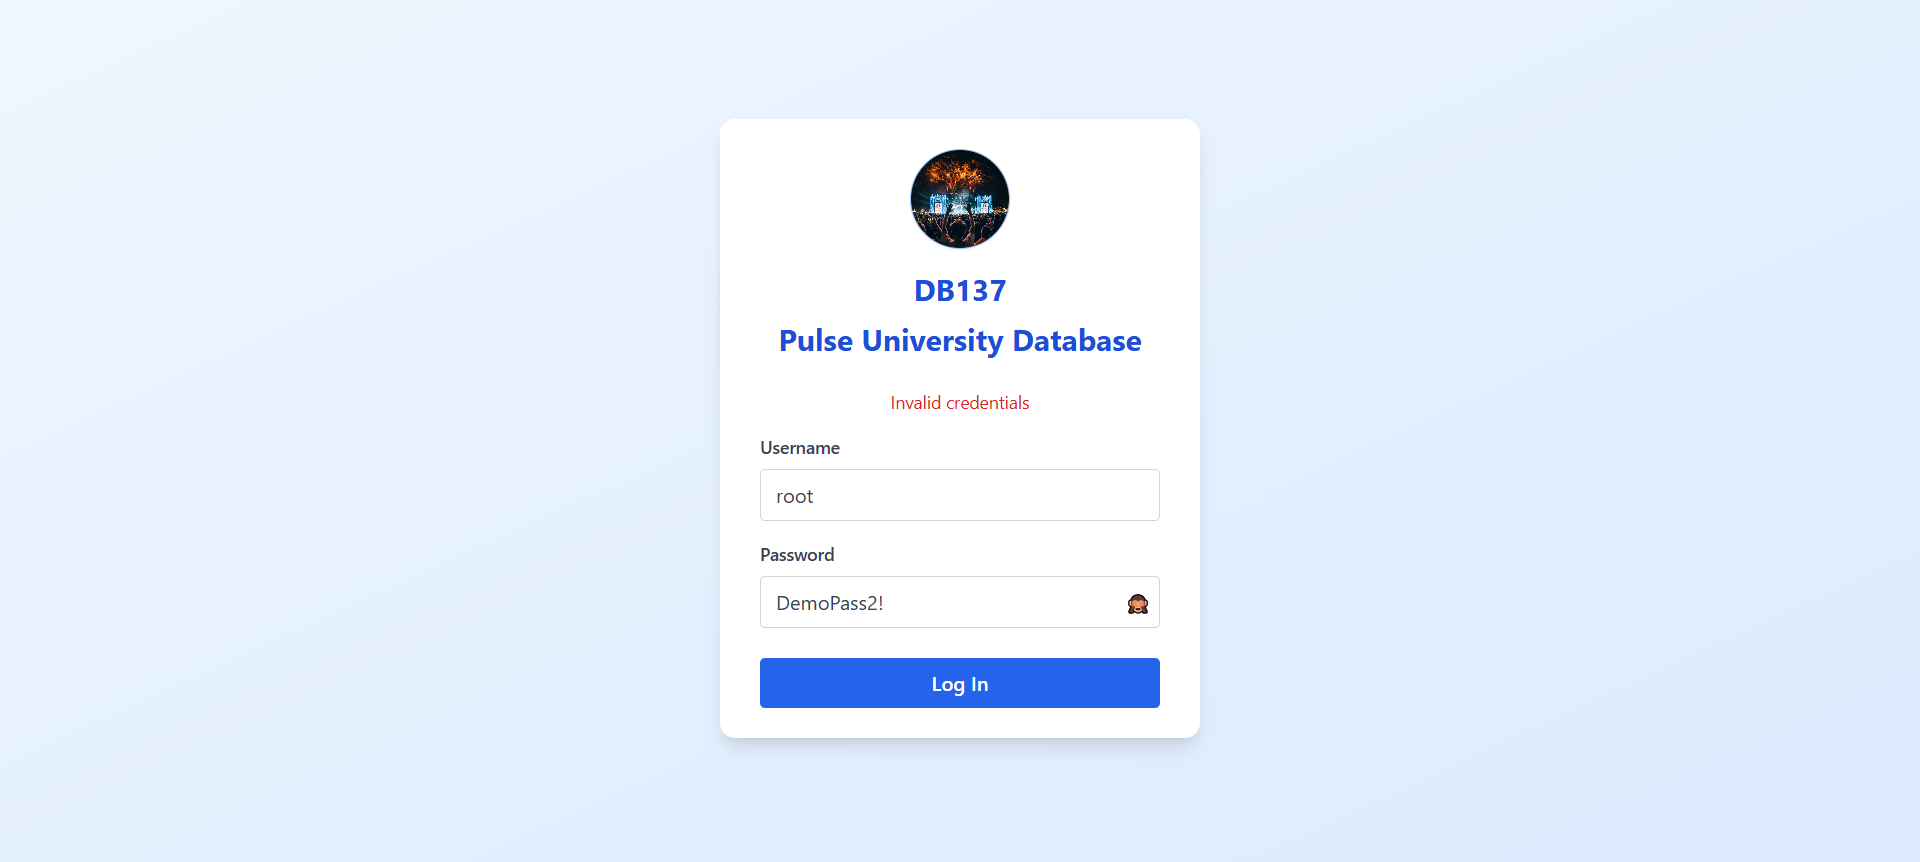
\includegraphics[width=0.95\linewidth]{Login.png}
    \caption{Σελίδα Σύνδεσης — υποστηρίζονται έλεγχος credentials, οπτική ανατροφοδότηση και αποθήκευση token.}
\end{figure}

\vspace{1.5cm}
\begin{figure}[H]
    \centering
    
\includegraphics[width=0.95\linewidth]{Logout.png}
    \caption{Σελίδα Αποσύνδεσης — καθαρισμός session και προσωπoποιημένο μήνυμα αποχαιρετισμού.}
\end{figure}

\clearpage
\begin{figure}[H]
    \centering
    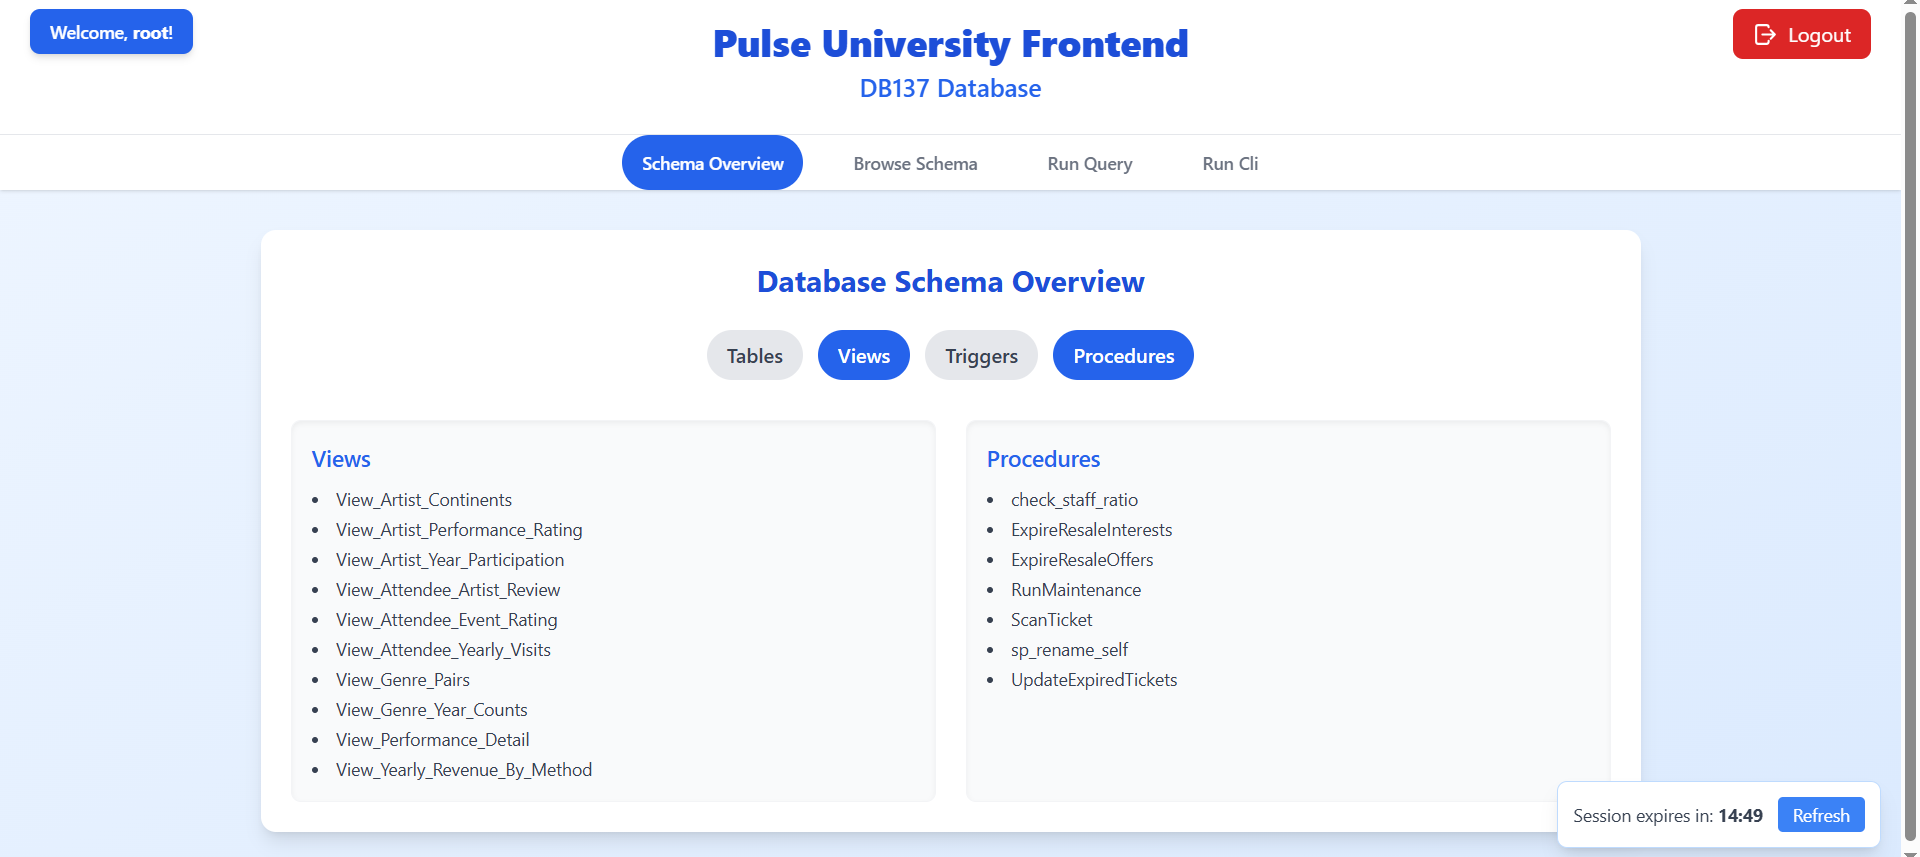
\includegraphics[width=0.95\linewidth]{Schema Overview Tab.png}
    \caption{Schema Overview Tab — εμφάνιση των πινάκων, views, triggers και procedures της βάσης.}
\end{figure}

\vspace{1.5cm}
\begin{figure}[H]
    \centering
    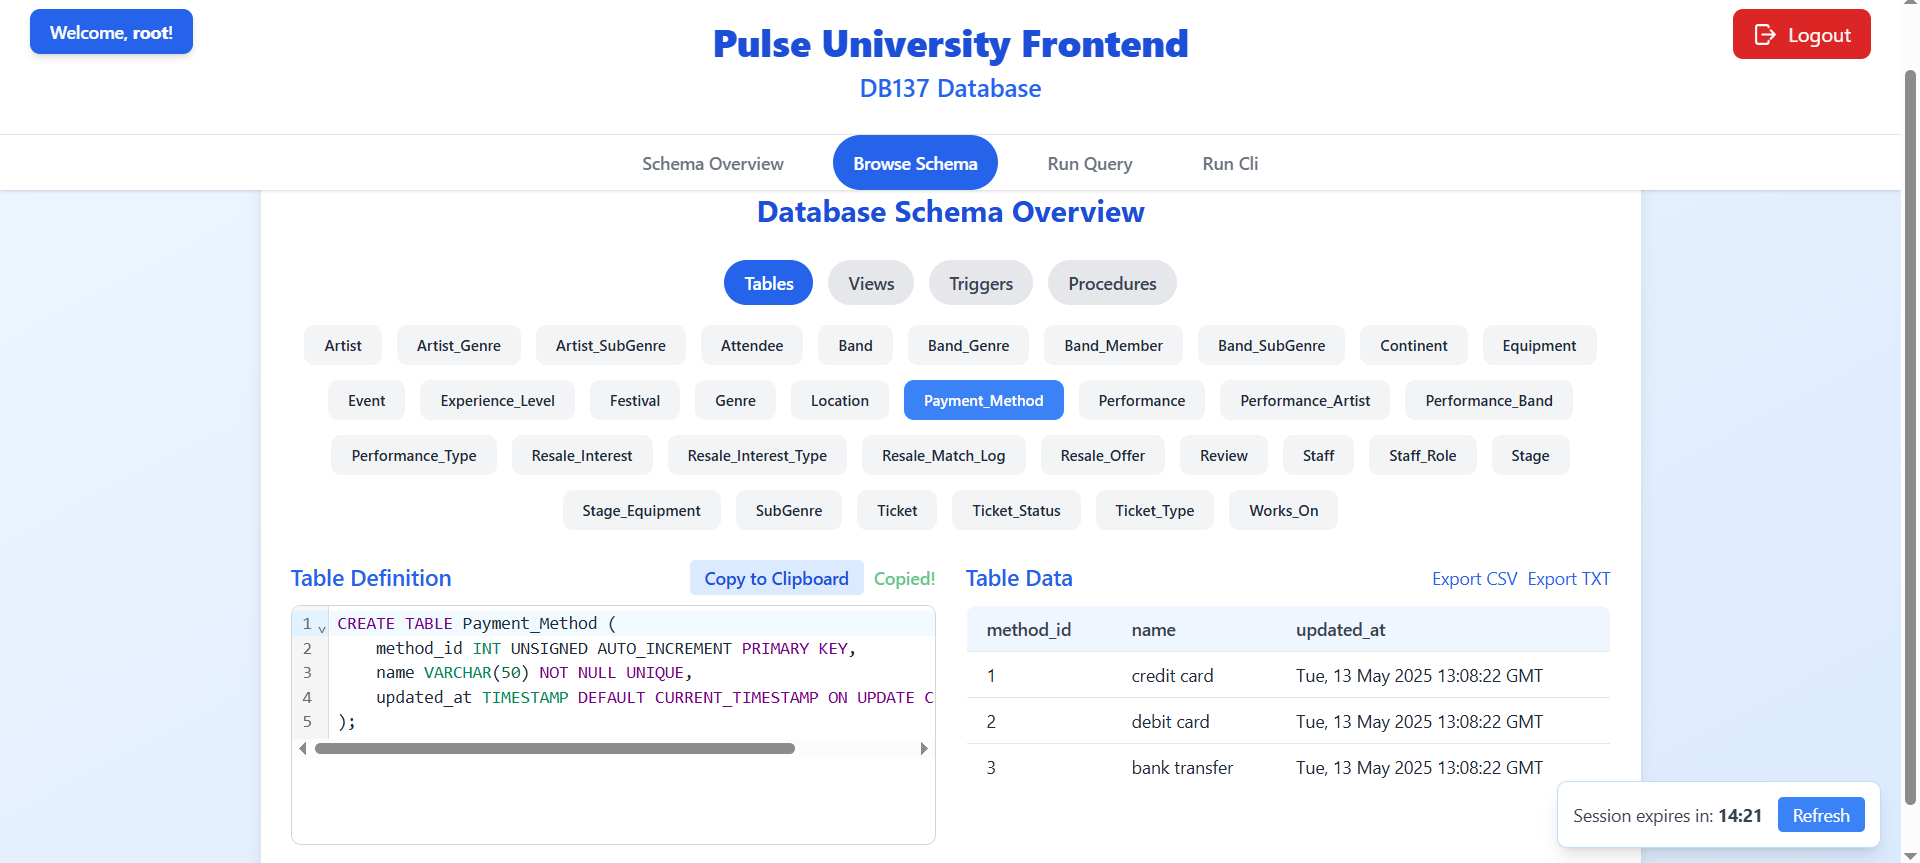
\includegraphics[width=0.95\linewidth]{Browse Tab.png}
    \caption{Browse Tab — εξερεύνηση δεδομένων πίνακα, προβολή ορισμών και δυνατότητα εξαγωγής.}
\end{figure}

\clearpage
\begin{figure}[H]
    \centering
    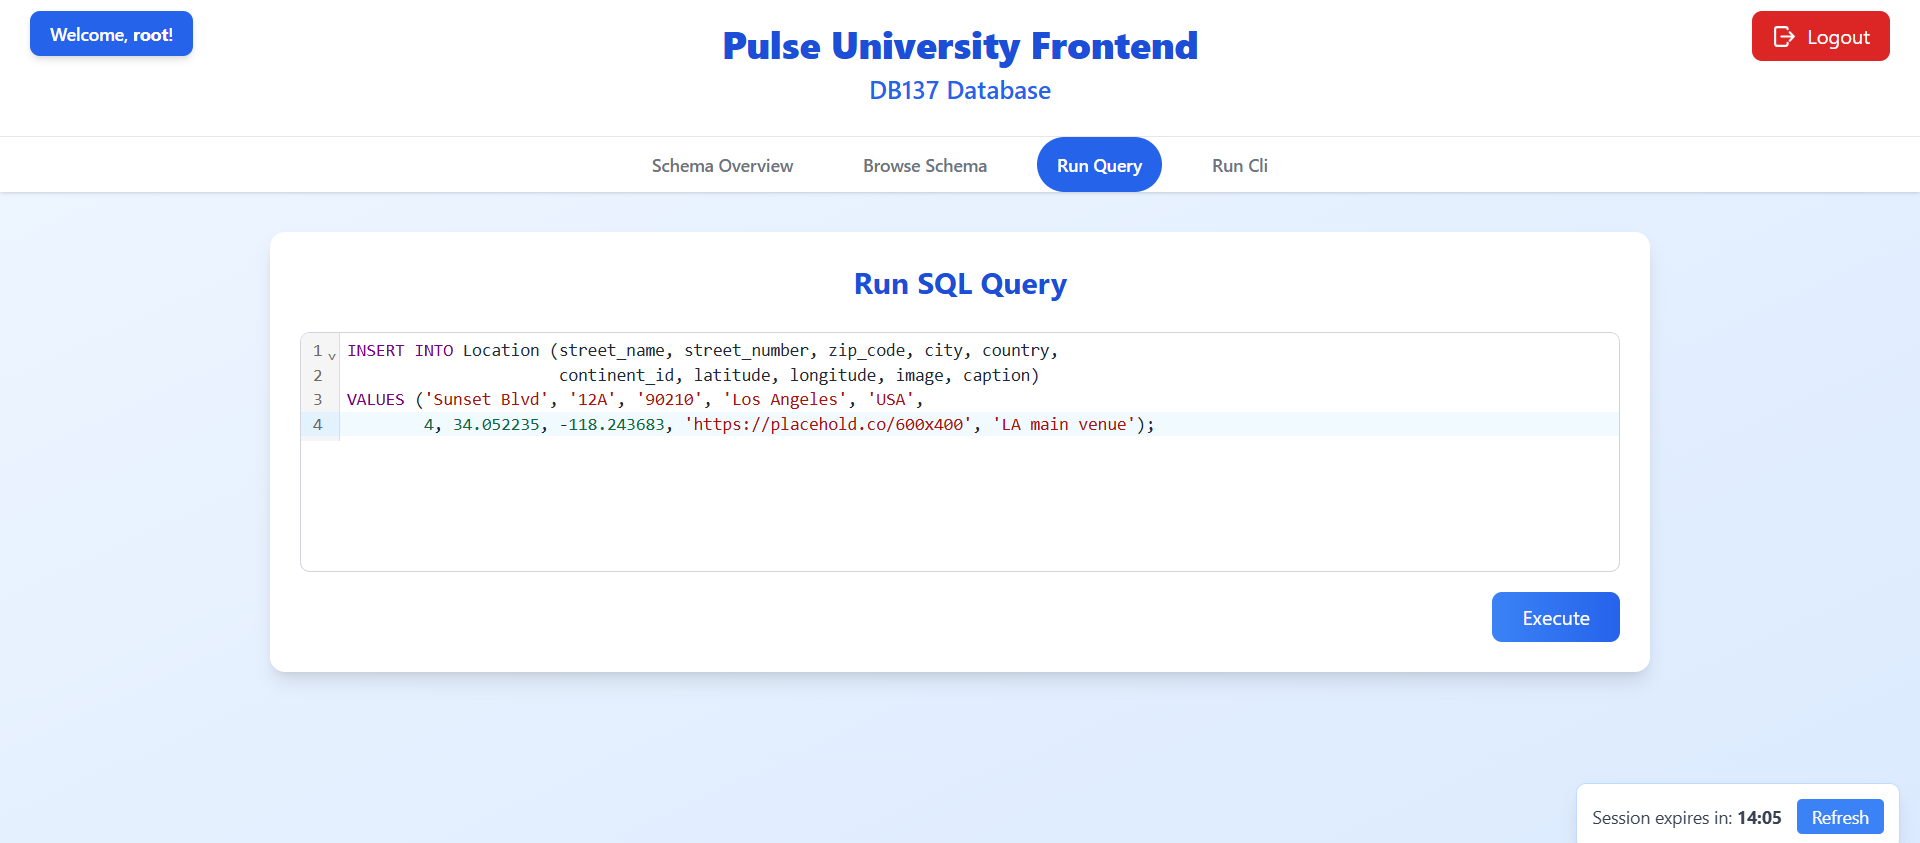
\includegraphics[width=0.95\linewidth]{Query Tab.png}
    \caption{Run Query Tab — εκτέλεση ερωτημάτων SQL με editor και προβολή αποτελεσμάτων.}
\end{figure}

\vspace{1.5cm}
\begin{figure}[H]
    \centering
    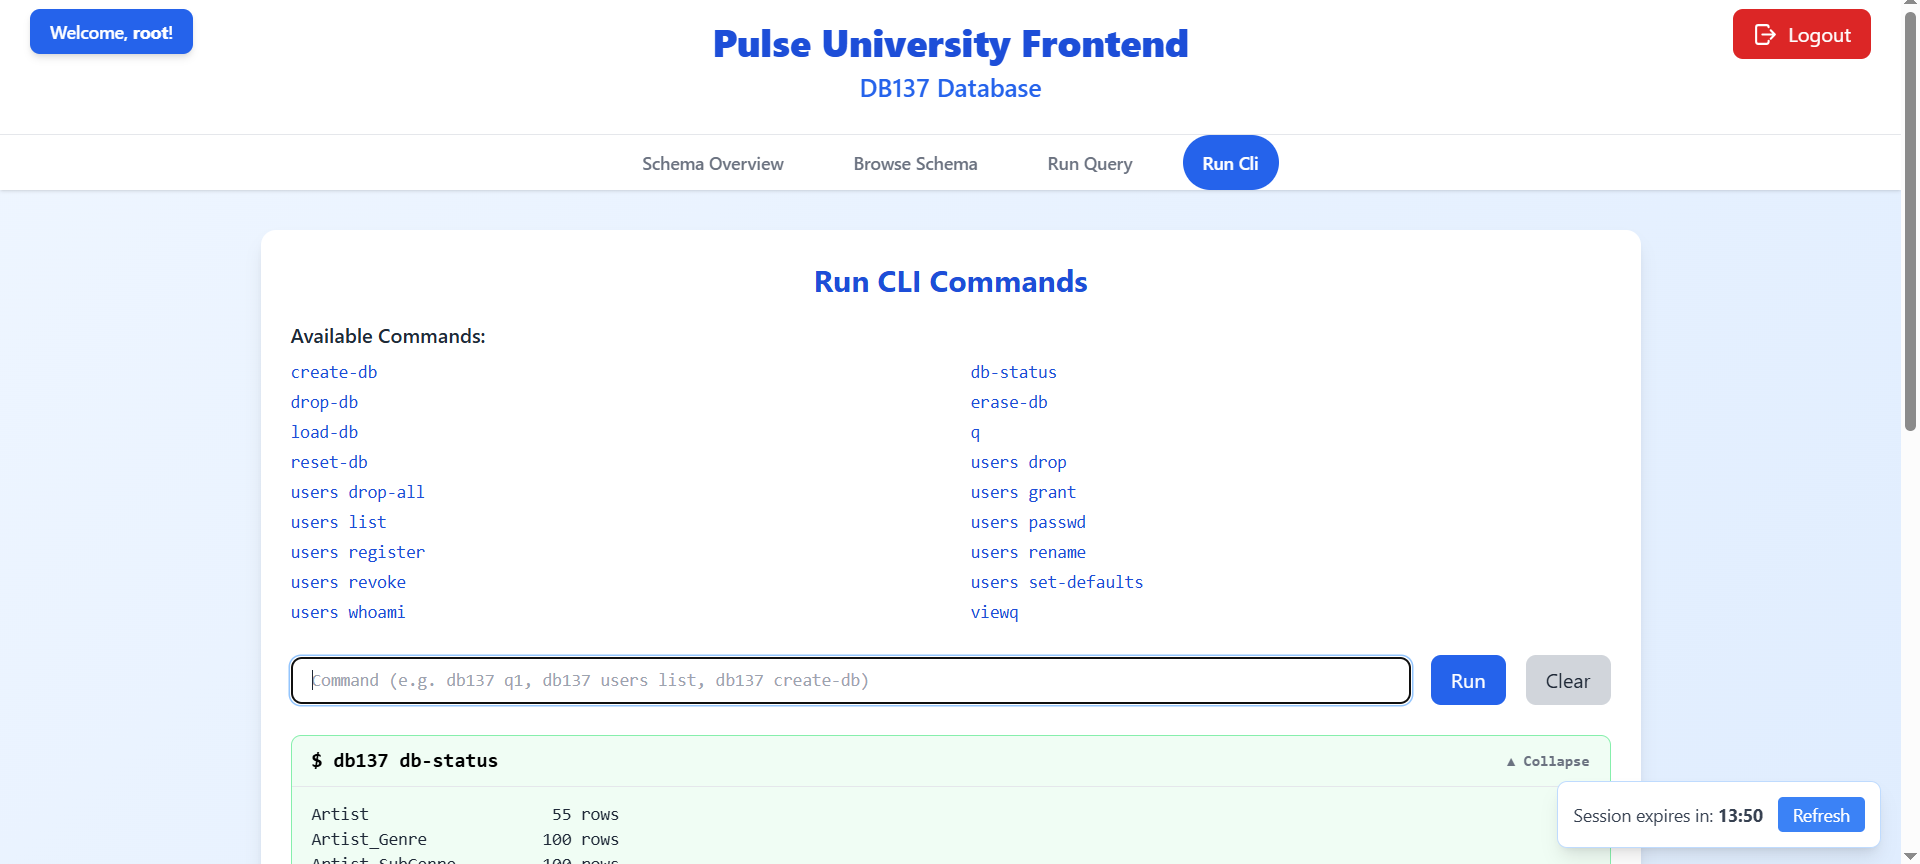
\includegraphics[width=0.95\linewidth]{CLI Tab.png}
    \caption{Run CLI Tab — υποστήριξη εντολών CLI, λίστα διαθέσιμων επιλογών και ιστορικό αποτελεσμάτων.}
\end{figure}


% ─────────────── 8. Οδηγίες Εγκατάστασης & Χρήση Εργαλείων AI ───────────────
\clearpage
\section{Οδηγίες Εγκατάστασης \& Χρήση Εργαλείων AI}

\subsection{Οδηγίες Εγκατάστασης}

\subsubsection{Schema}
Η εγκατάσταση του σχήματος της βάσης δεδομένων πραγματοποιείται με την εντολή:
\begin{center}
\texttt{db137 create-db}
\end{center}
η οποία εκτελεί διαδοχικά τα ακόλουθα SQL αρχεία:
\begin{itemize}
    \item \texttt{install.sql}: Ορισμός του πλήρους σχήματος και όλων των πινάκων.
    \item \texttt{indexing.sql}: Προσθήκη δεικτών βελτιστοποίησης.
    \item \texttt{procedures.sql}: Αποθηκευμένες διαδικασίες (π.χ. ticket scanning, maintenance).
    \item \texttt{triggers.sql}: Triggers για ελέγχους συνέπειας και λογικής.
    \item \texttt{views.sql}: Views που αντιστοιχούν σε graded queries.
\end{itemize}
Απαιτείται η ορθή ρύθμιση των μεταβλητών περιβάλλοντος στο αρχείο \texttt{.envrc}:
\begin{itemize}
    \item \texttt{DB\_ROOT\_USER}, \texttt{DB\_ROOT\_PASS}: root credentials.
    \item \texttt{DB\_HOST}, \texttt{DB\_PORT}, \texttt{DB\_NAME}: πληροφορίες σύνδεσης.
\end{itemize}

Προβλήματα που ενδέχεται να παρουσιαστούν:
\begin{itemize}
    \item \textbf{DB Connection Error}: λανθασμένα credentials ή host.
    \item \textbf{Privileges Error}: ο χρήστης δεν διαθέτει απαραίτητα δικαιώματα (π.χ. DROP/CREATE).
    \item \textbf{Syntax Error σε SQL αρχείο}: εντοπίζεται μέσω \texttt{ClickException}, με αναφορά γραμμής.
\end{itemize}

\subsubsection{CLI}

Η εγκατάσταση της γραμμής εντολών \texttt{db137} πραγματοποιείται αποκλειστικά σε \textbf{Linux ή WSL περιβάλλον}. Τα βήματα είναι τα εξής:

\paragraph{Α. Εξαρτήσεις}
\begin{itemize}
    \item \textbf{Python} ≥ 3.10
    \item \textbf{Βιβλιοθήκες Python:}
\begin{verbatim}
pip install --user click mysql-connector-python
\end{verbatim}
\end{itemize}

\paragraph{Β. Ορισμός αρχείου εγκατάστασης}
Δημιουργείται αρχείο \texttt{pyproject.toml} στο project root με το εξής περιεχόμενο:

\begin{verbatim}
[project]
name = "db137"
version = "0.1"
description = "Pulse University Database Helper CLI"
requires-python = ">=3.8"
dependencies = [
    "click",
    "mysql-connector-python",
]
[project.scripts]
db137 = "cli.db137:cli"
\end{verbatim}

\paragraph{Γ. Τοπική Εγκατάσταση (Editable)}
Από τον root φάκελο του project:

\begin{verbatim}
pip uninstall db137      # προαιρετικά
pip install --user -e .
\end{verbatim}

Αυτό δημιουργεί το εκτελέσιμο \texttt{db137} στο \texttt{\$HOME/.local/bin/db137}.

\paragraph{Δ. Ρύθμιση Shell}
Για να λειτουργεί η εντολή \texttt{db137} από οπουδήποτε:

\begin{verbatim}
export PATH="$HOME/.local/bin:$PATH"
source ~/.bashrc  # ή ~/.zshrc
which db137        # έλεγχος επιτυχίας
\end{verbatim}

\paragraph{Ε. Ρύθμιση Περιβάλλοντος μέσω \texttt{.envrc}}
Ορίζονται οι απαιτούμενες μεταβλητές:

\begin{verbatim}
export DB_ROOT_USER=$(echo -n 'root' | tr -d '')
export DB_ROOT_PASS=$(echo -n 'yourpassword' | tr -d '')
export PYTHONPATH=$PWD
export DB_HOST='localhost'
export DB_NAME='pulse_university'
export DB_PORT=3306
\end{verbatim}

Ενεργοποίηση:

\begin{verbatim}
direnv allow
\end{verbatim}

\paragraph{ΣΤ. Αντιμετώπιση Προβλημάτων}
\begin{itemize}
    \item \textbf{MySQL connection fails}:
    \begin{verbatim}
    sudo service mysql status
    sudo service mysql start
    \end{verbatim}

    \item \textbf{Blank DB\_ROOT\_USER or PASS}: Συνήθως σημαίνει ότι το \texttt{.envrc} δεν έχει φορτωθεί. Εκτελέστε:
    \begin{verbatim}
    direnv allow
    echo $DB_ROOT_USER
    \end{verbatim}

    \item \textbf{\texttt{db137: command not found}}: Προσθέστε το \texttt{\$HOME/.local/bin} στο \texttt{PATH}, κάντε \texttt{source ~/.bashrc} και ελέγξτε με \texttt{which db137}.

    \item \textbf{FileNotFoundError για SQL αρχεία}: Βεβαιωθείτε ότι έχετε δηλώσει σωστά το \texttt{--sql-dir}, π.χ.:
    \begin{verbatim}
    db137 create-db --sql-dir sql --database pulse_university
    \end{verbatim}
\end{itemize}

\paragraph{Ζ. Καθαρισμός Cache και Εγκαταστάσεων (προαιρετικά)}
\begin{verbatim}
find . -type d -name '__pycache__' -exec rm -r {} +
rm -rf db137.egg-info/
\end{verbatim}

\paragraph{Η. Εκτέλεση Ελέγχων CLI (Manual Testing)}
\begin{verbatim}
bash test/test_cli.sh
\end{verbatim}

Τα αποτελέσματα αποθηκεύονται στο \texttt{test/test\_cli\_results.txt}.

\clearpage
\subsubsection{Frontend}

Η εγκατάσταση του frontend γίνεται εντός περιβάλλοντος \textbf{WSL} και περιλαμβάνει την υλοποίηση SPA διεπαφής με χρήση \texttt{React}, \texttt{Vite}, \texttt{Tailwind CSS} και backend σε \texttt{Flask}.

\paragraph{Α. Εγκατάσταση Node.js μέσω \texttt{nvm}}
\begin{verbatim}
curl -o- https://raw.githubusercontent.com/nvm-sh/nvm/v0.39.7/install.sh | bash
source ~/.bashrc
nvm install 20.11.0
nvm use 20.11.0
\end{verbatim}

\paragraph{Β. Εγκατάσταση Εξαρτήσεων Frontend}
Από τον φάκελο \texttt{frontend/}:

\begin{verbatim}
npm install
npm install --save-dev @vitejs/plugin-react
npm install @uiw/react-codemirror @codemirror/lang-sql
\end{verbatim}

\paragraph{Γ. Εγκατάσταση Flask Backend για Local χρήση}
\begin{verbatim}
pip install flask flask-cors mysql-connector-python
\end{verbatim}

\paragraph{Δ. Εκκίνηση Frontend και Backend (σε ξεχωριστά terminals)}
\begin{verbatim}
npm run dev                          # Frontend (http://localhost:3000)
python3 frontend/src/api/serve.py   # Backend (port 8000)
\end{verbatim}

\paragraph{Ε. Αντιμετώπιση Κοινών Προβλημάτων}
\begin{itemize}
    \item \textbf{ERR\_INVALID\_ARG\_TYPE: Received undefined} \\
    Προκαλείται από απουσία ή βλάβη του \texttt{node}. Επανεγκαταστήστε με \texttt{nvm}.

    \item \textbf{npm audit warnings} \\
    Αγνοούνται κατά την ανάπτυξη. Μην εκτελέσετε \texttt{npm audit fix --force} — υπάρχει κίνδυνος ασυμβατότητας με \texttt{Vite}.

    \item \textbf{Διαδρομές τύπου OneDrive ή προβλήματα δικαιωμάτων} \\
    Μετακινήστε το έργο εκτός \texttt{OneDrive}, π.χ. σε \texttt{C:\textbackslash Projects\ DB25\_137}.

    \item \textbf{Tailwind styles δεν εφαρμόζονται} \\
    Επιβεβαιώστε ότι το \texttt{index.css} περιλαμβάνει:
\begin{verbatim}
@tailwind base;
@tailwind components;
@tailwind utilities;
\end{verbatim}

    \item \textbf{Failed to resolve import "@/"} \\
    Ελέγξτε τα alias στο \texttt{vite.config.js} — πρέπει να αντιστοιχούν στον φάκελο \texttt{src/}.
\end{itemize}

\paragraph{Ζ. Σημειώσεις Περιβάλλοντος}
\begin{itemize}
    \item Το frontend χρησιμοποιεί \texttt{sessionStorage} για token authentication διάρκειας 15 λεπτών
    \item Όλες οι κλήσεις γίνονται προς το Flask backend στη θύρα \texttt{8000}
    \item Η δομή αρχείων και οι imports βασίζονται στο \texttt{vite.config.js} και το \texttt{tailwind.config.js}
\end{itemize}

\subsection{Βοηθητικά Εργαλεία Κώδικα}

Ο φάκελος \texttt{code/} περιέχει scripts για debugging, παραγωγή δεδομένων και συντήρηση του project:
\begin{itemize}
    \item \texttt{data\_generation/faker.py}: Εισάγει πλήρη και trigger-compliant δεδομένα απευθείας στη βάση.
    \item \texttt{data\_generation/faker\_sql.py}: Παράγει SQL queries με χρήση write helpers και αποθηκεύει στο \texttt{load.sql}.
    \item \texttt{code\_utils/qgen.py}: Δημιουργεί αρχεία \texttt{Q01.sql} έως \texttt{Q15.sql} και τα αντίστοιχα \texttt{Q01\_out.txt}, αν δεν υπάρχουν ή είναι κενά.
    \item \texttt{code\_utils/fixeof.py}: Εισάγει μια κενή γραμμή στο τέλος σημαντικών αρχείων για αποφυγή σφαλμάτων κατά το parsing.
    \item \texttt{code\_utils/dropgen.py}: Προσθέτει στα SQL αρχεία που σχετίζονται με το σχήμα (π.χ. \texttt{install}, \texttt{triggers}) ένα \texttt{DROP IF EXISTS} block πριν από δημιουργία των αντίστοιχων entities, triggers, κ.λπ.
    \item \texttt{organization/struct.py}: Σαρώνει τη δομή του project (πλην των .gitignore) και την τυπώνει στο \\ \texttt{docs/oragnization/project\_structure.txt} με χρήση της εντολής \texttt{tree}.
    \item \texttt{runall.py}: Ολιστικό script που εκτελεί όλα τα παραπάνω, σε σωστή σειρά.
\end{itemize}

\subsection{Χρήση Εργαλείων AI}

Κατά την υλοποίηση της εργασίας αξιοποιήθηκε το \textbf{ChatGPT Plus (GPT-4)} ως εργαλείο Τεχνητής Νοημοσύνης για καθοδήγηση, ενίσχυση παραγωγικότητας και παραγωγή κώδικα σε συγκεκριμένα υποστηρικτικά σημεία.

\paragraph*{Α. Παραγωγή Python \& JavaScript Κώδικα}~\\

Το AI παρήγαγε έτοιμο και προσαρμόσιμο κώδικα για:
\begin{itemize}
    \item Shell scripts για CLI testing: \texttt{test\_cli.sh}.
    \item Bοηθητικά Python scripts: \texttt{dropgen.py}, \texttt{fixeof.py}, \texttt{qgen.py}, \texttt{runall.py}.
    \item Σύλληψη και ενσωμάτωση generating Scripts (π.χ. \texttt{faker.py}).
    \item Πολύπλοκα python modules, πέραν της εμβέλειας του μαθήματος, όπως \texttt{manager.py} και \texttt{serve.py}.
    \item JavaScript και React modules για την οργάνωση του frontend (React Tabs, CLI Terminal, CodeMirror Editor).
\end{itemize}
Όλα τα παραπάνω επανελέγχθηκαν, διορθώθηκαν ή επεκτάθηκαν από την ομάδα ώστε να διασφαλιστεί η τεχνική πληρότητα, η ασφάλεια και η συμβατότητα με το σύνολο της εφαρμογής.

\paragraph{Β. Υποστήριξη Debugging και Εγκατάστασης}
\begin{itemize}
    \item Ανάλυση σφαλμάτων CLI και React κατά την εγκατάσταση (π.χ. \texttt{ModuleNotFoundError}, \texttt{import failures}, \texttt{nvm issues}).
    \item Αντιμετώπιση προβλημάτων σε \texttt{vite.config.js}, \texttt{tailwind.config.js}, \texttt{.envrc} περιβάλλον.
    \item Εντοπισμός λαθών σε privileges, triggers, procedures και άλλους περιορισμούς.
\end{itemize}

\paragraph{Γ. Μορφοποίηση και Τεκμηρίωση}
\begin{itemize}
    \item Βοήθεια στη διαμόρφωση των αρχείων \texttt{README.md}.
    \item Εξαγωγή σε markdown / LaTeX.
\end{itemize}

\textbf{Σημείωση}: Όλες οι υλοποιήσεις που σχετίζονται με schema, queries, triggers, constraints και views σε SQL έγιναν χειροκίνητα από την ομάδα, με μόνο συντακτική επιβεβαίωση από την AI. Δεν παραδόθηκε ή χρησιμοποιήθηκε παραγόμενος SQL κώδικας.


\end{document}
